\documentclass[a4paper,11pt,msc]{SBU}
% در این فایل، دستورها و تنظیمات مورد نیاز، آورده شده است.
%-------------------------------------------------------------------------------------------------------------------

\usepackage{stmaryrd}
\usepackage{amssymb,amsmath,amsthm}
%ایجاد فرورفتگی در اولین پاراگراف هر بخش
\usepackage{indentfirst}
% بسته‌ای برای تنطیم حاشیه‌های بالا، پایین، چپ و راست صفحه
\usepackage[top=30mm, bottom=30mm, left=25mm, right=35mm]{geometry}
% بسته‌‌ای برای ظاهر شدن شکل‌ها و تصاویر متن
\usepackage{graphicx}
% بسته‌ای برای رسم کادر
\usepackage{framed} 
% بسته‌‌ای برای چاپ شدن خودکار تعداد صفحات در صفحه «معرفی پایان‌نامه»
\usepackage{lastpage}
% بسته‌‌ای برای ایجاد دیاگرام‌های مختلف
\usepackage[all]{xy}
\usepackage{tikz}
\usetikzlibrary{topaths}
\tikzset{terminal/.style={
		% The shape:
		rectangle ,minimum size =6mm,rounded corners=4mm,
		% The rest
		%very thick,draw=black!50,
		top color=green!10,bottom color=green!40,
		font=\ttfamily}}
	
	\usepackage{float}
	
	
% بسته‌ و دستوراتی برای ایجاد لینک‌های رنگی با امکان جهش
\usepackage[linktocpage=true,colorlinks,pagebackref=true,linkcolor=blue,citecolor=magenta]{hyperref}
% چنانچه قصد پرینت گرفتن نوشته خود را دارید، خط بالا را غیرفعال و  از دستور زیر استفاده کنید چون در صورت استفاده از دستور زیر‌‌، 
% لینک‌ها به رنگ سیاه ظاهر خواهند شد که برای پرینت گرفتن، مناسب‌تر است
%\usepackage[pagebackref=false]{hyperref}
%بسته‌ی لازم برای مراجع
\usepackage[nonamebreak,square]{natbib}
% بسته‌ لازم برای تنظیم سربرگ‌ها
\usepackage{fancyhdr}
% بسته‌ای برای ظاهر شدن «مراجع» و «نمایه» در فهرست مطالب
%\usepackage[nottoc]{tocbibind}


% دستورات مربوط به ایجاد نمایه
\usepackage{makeidx}
\makeindex
%%%%%%%%%%%%%%%%%%%%%%%%%%
% فراخوانی بسته زی‌پرشین و تعریف قلم فارسی و انگلیسی
\usepackage{xepersian}
\settextfont[Scale=1.15]{XB Niloofar}
%\setiranicfont[Scale=1]{PersianModern-Oblique}
\setiranicfont[Scale=1.15]{XB Zar Oblique}
% چنانچه می‌خواهید اعداد در فرمول‌ها، انگلیسی باشد، خط زیر را غیرفعال کنید
%\setdigitfont{Yas}
\setdigitfont[Scale=.85]{Persian Modern}
%\setdigitfont[Scale=1.1]{XB Zar}
%\KashidaOn
%تنظیم فاصله‌ی خطوط و پاراگراف‌ها
\linespread{1.3}
\setlength{\parskip}{1ex plus 0.5ex minus 0.2ex}
%%%%%%%%%%%%%%%%%%%%%%%%%%
% تعریف قلم‌های فارسی و انگلیسی اضافی برای استفاده در بعضی از قسمت‌های متن
\defpersianfont\nastaliq[Scale=1.50]{XB Niloofar}
\defpersianfont\chapternumber[Scale=3.02]{XB Niloofar}
\defpersianfont\titr[Scale=1.02]{XB Titre}
\defpersianfont\dav[Scale=2]{B Davat}
%%%%%%%%%%%%%%%%%%%%%%%%%%
% دستوری برای حذف کلمه «چکیده»
\renewcommand{\abstractname}{}
% دستوری برای حذف کلمه «abstract»
\renewcommand{\latinabstract}{}
% دستوری برای تغییر نام کلمه «اثبات» به «برهان»
\renewcommand\proofname{\textbf{برهان}}
% دستوری برای تغییر نام کلمه «کتاب‌نامه» به «مراجع»
\renewcommand{\bibname}{مراجع}
%استفاده از کلمه‌ی نمودار به جای شکل
\renewcommand{\figurename}{نمودار}
% دستوری برای تعریف واژه‌نامه انگلیسی به فارسی
\newcommand\persiangloss[2]{#1\dotfill\lr{#2}\\}
% دستوری برای تعریف واژه‌نامه فارسی به انگلیسی 
\newcommand\englishgloss[2]{#2\dotfill\lr{#1}\\}
%%%%%%%%%%%%%%%%%%%%%%%%%%
% تعریف و نحوه ظاهر شدن عنوان قضیه‌ها، تعریف‌ها، مثال‌ها و ...
\theoremstyle{definition}
\newtheorem{definition}{تعریف}[section]
%\newtheorem{deduct}[definition]{}
\newtheorem{theorem}[definition]{قضیه}
\newtheorem{lemma}[definition]{لم}
\newtheorem{proposition}[definition]{گزاره}
\newtheorem{corollary}[definition]{نتیجه}
\newtheorem{remark}[definition]{ملاحظه}
\newtheorem{example}[definition]{مثال}
%%%%%%%%%%%%%%%%%%%%%%%%%%
% تعریف دستورات جدید برای خلاصه نویسی و راحتی کار در هنگام تایپ فرمول‌های ریاضی
\newcommand{\mA}{\mathcal{A}}% مجموعه‌ی عامل‌ها
\newcommand{\mB}{\mathcal{B}}% زیرمجموعه‌ای از عامل‌ها
\newcommand{\mL}{\mathcal{L}}% زبان
\newcommand{\mF}{\mathcal{F}}% سیگما جبر
\newcommand{\mP}{\mathcal{P}}% تخصیص احتمالاتی
\newcommand{\mK}{\mathcal{K}}% منطق K
\newcommand{\mS}{\mathcal{S}}% منطق S5
\newcommand{\mbbP}{\mathbb{P}}% مجموعه‌ی گزاره‌های اتمی
\newcommand{\mbbQ}{\mathbb{Q}}% مجموعه‌ی اعداد گویا
\newcommand{\mbbM}{\mathbb{M}}% مجموعه‌ی مدل‌های شناختی احتمالاتی
\newcommand{\mbbK}{\mathbb{K}}% کلاس مدل‌های کریپکی
\newcommand{\mbbS}{\mathbb{S}}% کلاس مدل‌های شناختی
\newcommand{\mbP}{\mathbf{P}}% نماد تابعی احتمالاتی
\newcommand{\xra}{\xrightarrow}
\newcommand{\scr}{\scriptscriptstyle}
\newcommand{\bp}{\begin{proof}}
	\newcommand{\ep}{\end{proof}}
%\newcommand{\close}{\begin{latin}\noindent $\square$ \end{latin}}
%%%%%%%%%%%%%%%%%%%%%%%%%%%%%%%%%%%%%%%%%%%
%تعریف اعداد لاتین برای زمانی که از اعداد فارسی در متن استفاده می‌کنیم
\def\0{\textrm{\lr{0}}}
\def\1{\textrm{\lr{1}}}
\def\2{\textrm{\lr{2}}}
\def\3{\textrm{\lr{3}}}
\def\4{\textrm{\lr{4}}}
\def\5{\textrm{\lr{5}}}
%%%%%%%%%%%%%%%%%%%%%%%%%%%%%%%%%%%%%%%%%%%
\def\reduction{تحویل}
\def\observation{مشاهده‌محور}
\def\prior{پیشینی}
%%%%%%%%%%%%%%%%%%%%%%%%%%%%%%%%%%%%%%%%%%%
% براساس نسخه‌های از ۱.۲.۵ به بعد بسته‌ی bidi در توابع زیر باید توجه داشت:
% که l یعنی شروع نوشتار از ابتدای خط یا جعبه،
% و r یعنی شروع نوشتار از انتهای خط یا جعبه، 
% و s یعنی شروع نوشتار از وسط خط یا جعبه.
\newdimen\xleftright
\xleftright=\textwidth
\advance \xleftright by -10.5cm
\newcommand{\leftright}[3]{%
	\noindent
	\makebox[4 cm][r]{#1}
	\makebox[\xleftright][s]{}
	\makebox[5.5 cm][l]{#2}
	\makebox[1 cm][l]{#3}%
}
\newcommand{\leftrightb}[2]{%
	\noindent
	\makebox[4 cm][r]{#1}
	\makebox[\xleftright][s]{}
	\makebox[6.5 cm][l]{#2}%
}
\newcommand{\semanticsa}[2]{%
	\noindent
	\makebox[4.3 cm][r]{#1}
	\makebox[\xleftright][c]{اگر و فقط اگر}
	\makebox[6.2 cm][l]{#2}%
}
\newcommand{\semanticsb}[2]{%
	\noindent
	\makebox[3.5 cm][l]{#1}
	\makebox[\xleftright][c]{اگر و فقط اگر}
	\makebox[7 cm][r]{#2}%
}
%%%%%%%%%%%%%%%%%%%%%%%%%%%%
% دستورهایی برای سفارشی کردن سربرگ صفحات
\csname@twosidetrue\endcsname
\pagestyle{fancy}
\fancyhf{} 
\fancyhead[RE,LO]{\thepage}
\fancyhead[LE]{\small\iranicfamily\leftmark}
\fancyhead[RO]{\small\iranicfamily\rightmark}
\renewcommand{\chaptermark}[1]{%
	\markboth{\thechapter.\ #1}{}}
%%%%%%%%%%%%%%%%%%%%%%%%%%%%%
% دستورهایی برای سفارشی کردن صفحات اول فصل‌ها
\makeatletter
\newcommand\mycustomraggedright{%
	\if@RTL\raggedleft%
	\else\raggedright%
	\fi}
\def\@part[#1]#2{%
	\ifnum \c@secnumdepth >-2\relax
	\refstepcounter{part}%
	\addcontentsline{toc}{part}{\thepart\hspace{1em}#1}%
	\else
	\addcontentsline{toc}{part}{#1}%
	\fi
	\markboth{}{}%
	{\centering
		\interlinepenalty \@M
		\ifnum \c@secnumdepth >-2\relax
		\huge\bfseries \partname\nobreakspace\thepart
		\par
		\vskip 20\p@
		\fi
		\Huge\bfseries #2\par}%
	\@endpart}
\def\@makechapterhead#1{%
	\vspace*{-30\p@}%
	{\parindent \z@ \mycustomraggedright %\@mycustomfont
		\ifnum \c@secnumdepth >\m@ne
		\if@mainmatter
		
		\huge\bfseries \@chapapp\space {\chapternumber\thechapter}
		\par\nobreak
		\vskip 20\p@
		\fi
		\fi
		\interlinepenalty\@M 
		\Huge \bfseries #1\par\nobreak
		\vskip 120\p@
}}
\makeatother
\begin{document}
\frontmatter
%%%%%%%%%%%%%%%%%%%%%%%%%%%%%%%%%%%%%%%%%
%صفحه‌ی بسم الله
%\thispagestyle{empty}
%\centerline{{\includegraphics[width=9 cm]{*}}}
%\newpage
%\thispagestyle{empty}
%\clearpage
%~~~
%%%%%%%%%%%%%%%%%%%%%%%%%%%%%%%%%%%%%%%%%




\newcommand{\mychapter}[1]{%
	\chapter*{#1}
	\addcontentsline{toc}{chapter}{#1}
	\markboth{#1}{}
}

\newcommand{\mysection}[1]{%
	\section*{#1}
	\addcontentsline{toc}{section}{#1}
}



\clearpage
\pagenumbering{adadi}
% در این فایل، عنوان پایان‌نامه، مشخصات خود، متن تقدیمی‌، ستایش، سپاس‌گزاری و چکیده پایان‌نامه را به فارسی، وارد کنید.
% توجه داشته باشید که جدول حاوی مشخصات پایان‌نامه/رساله و همچنین، مشخصات داخل آن، به طور خودکار، درج می‌شود.
%%%%%%%%%%%%%%%%%%%%%%%%%%%%%%%%%%%%
% دانشگاه خود را وارد کنید
\university{شهید بهشتی}
% دانشکده، آموزشکده و یا پژوهشکده  خود را وارد کنید
\faculty{حقوق }
% گروه آموزشی خود را وارد کنید
\degree {کارشناسی ارشد} 
% گروه آموزشی خود را وارد کنید
\subject{دانشکده حقوق}
% گرایش خود را وارد کنید
\field{حقوق محیط زیست}
% عنوان پایان‌نامه را وارد کنید
\title{تاثیر تغییرات اقلیمی بر حق بر آینده سبز}
% نام استاد(ان) راهنما را وارد کنید
\firstsupervisor{دکتر جنت بلیک}
%\secondsupervisor{استاد راهنمای دوم}
% نام استاد(دان) مشاور را وارد کنید. چنانچه استاد مشاور ندارید، دستور پایین را غیرفعال کنید.
\firstadvisor{دکتر باقر انصاری}
%\secondadvisor{استاد مشاور دوم}
% نام پژوهشگر را وارد کنید
\name{محمد مهدی}
% نام خانوادگی پژوهشگر را وارد کنید
\surname{وزیری}
% تاریخ پایان‌نامه را وارد کنید
\thesisdate{1397}
% کلمات کلیدی پایان‌نامه را وارد کنید
\keywords{تغییرات اقلیمی، آینده سبز، حقوق کودک، حقوق نسل های آینده}
% چکیده پایان‌نامه را وارد کنید
\fa-abstract{\noindent
نسل‌های گذشته و حاضر با دامن زدن به تغییرات‌اقلیمی، نظم و الگوی دما و بارش را در سطح کره زمین تغییر داده‌اند، به نحوی که پایداری و ثبات اقلیم دچار اختلال شده است. بازگشت اقلیم به وضعیت ثبات چیزی حدود ده هزار سال زمان نیاز خواهد داشت و این به معنای وجود چالش در رابطه بین نسل‌های حاضر و آینده است. 
در این میان، باید پرسید که تغییرات‌اقلیمی چه تاثیری بر ذینفعان حق بر آینده سبز می‌گذارد. همچنین تعهد نسل‌های حاضر در برابر حق بر آینده سبز در ساختار حقوق بین‌الملل محیط‌زیست چیست؟
%تعهدات مختلفی در کنوانسیون‌های حقوق بین‌الملل محیط‌زیست برای مقابله با این پدیده تدارک دیده شده است، ماهیت نرم این تعهدات و منفعت‌طلبی دولت‌ها با تکیه بر اصل حاکمیت دولت‌ها، مانع شکل‌گیری اجماع بین‌المللی موثر در برابر این پدیده و حمایت از حق بر آینده سبز بوده است. \\
تغییر دما و بارش، با ایجاد محدودیت در دسترسی به منابع، کودکان را از نیاز‌های اساسی، حقوق خاص، حقوق مشارکتی  و زندگی در جامعه‌ای پایدار که حقوق اقتصادی، اجتماعی، فرهنگی، سیاسی و مدنی آنها تضمین شده باشد، محروم می‌نماید. کودکان و نسل‌های آینده، شهروندان آینده زمین هستند که حق آنها بر دریافت زمین به مثابه میراث مشترک بشریت در کمال صحت از نسل‌های حاضر، در حال نقض است. تغییرات‌اقلیمی با محدود نمودن منابع و تخریب آنها، آزادی انتخاب کودکان و نسل‌های آینده را تحدید می‌نماید.\\
جامعه بین‌المللی، در این حوزه با تاکید بر خیر مشترک، عدالت و جامعه ارزش‌های بنیادین بین‌المللی و با تکیه بر اصول همکاری، مسئولیت مشترک اما متفاوت و... توانسته گام‌های در مقابله با تغییرات‌اقلیمی در قالب کنوانسیون چارچوبی تغییرات‌اقلیمی کنوانسیون تنوع زیستی و دیگر اسناد بردارد. اما الزام‌آور نبودن این تعهدات در کنار رقابت اقتصادی دولت‌ها و اصل حاکمیت دولت‌ها در ساختار‌های قدیمی حقوق بین‌الملل از نتیجه بخش بودن این اقدامات کاسته، به نحوی که انتشار گاز‌های گلخانه‌ای روند افزایشی داشته و اجماع بین‌المللی در این حوزه با موفقیت کامل روبه‌رو نبوده است و آینده‌ای سبز را نوید نمی‌دهد. 
در فرایند نگارش سعی گردیده با رویکرد آینده‌نگرانه به موضوع نگریسته شود و از رهیافت ایده‌آلیستی در تببین آرمان‌های جامعه بین‌المللی و نقش آنها در تنظیم رابطه نسل حاضر با نسل‌های آینده استفاده شده است. }
\newpage
\thispagestyle{empty}
\vtitle
\newpage
\thispagestyle{empty}
\clearpage
~~~
\newpage
\thispagestyle{empty}
\ \\ \\ \\ \\ \\ \\ \\
{\dav
\begin{center}
كلية حقوق اعم از چاپ و تكثير، نسخه برداري ، ترجمه، اقتباس و ... از اين پايان نامه براي دانشگاه شهيد بهشتي محفوظ است.
 نقل  مطالب با ذكر مأخذ آزاد است.
\end{center}
}
\newpage
\thispagestyle{empty}
\clearpage
~~~
%\newpage
%\thispagestyle{empty}
%\centerline{{\includegraphics[width=20 cm]{replyrecord}}}
%\newpage
%\thispagestyle{empty}
%\clearpage
%~~~
\newpage
 % پایان‌نامه خود را تقدیم کنید!
\begin{acknowledgementpage}

\vspace{4cm}

{\nastaliq
{\Large
تقدیم به مادرم که بذرهای امیدواری می‌کارد، تا من درو کنم.

و تقدیم به عبدالحسین وهاب‌زاده، موسس مدارس طبیعت که دغدغه طبیعت و نسل‌های آینده را دارد.
\vspace{1.5cm}

\newdimen\xa
\xa=\textwidth
\advance \xa by -11cm
\hspace{\xa}
با مهر
}}
\end{acknowledgementpage}
\newpage
\thispagestyle{empty}
\clearpage
~~~
%%%%%%%%%%%%%%%%%%%%%%%%%%%%%%%%%%%%
%\newpage
\thispagestyle{empty}
% ستایش
\baselineskip=.750cm
\ \\ \\
 
{\nastaliq
%رسيدن، به دانش است و به كردار نیک...%
}\\
\vspace{.5cm}\\
{\scriptsize\nastaliq
{



«وَمِنَ النَّاسِ مَنْ یُعْجِبُکَ قَوْلُهُ فِی الْحَیَاةِ الدُّنْیَا وَیُشْهِدُ اللَّهَ عَلَىٰ مَا فِی قَلْبِهِ وَهُوَ أَلَدُّ الْخِصَامِ،(204) وَإِذَا تَوَلَّىٰ سَعَىٰ فِی الْأَرْضِ لِیُفْسِدَ فِیهَا وَ یُهْلِکَ الْحَرْثَ وَالنَّسْلَ  وَاللَّهُ لَا یُحِبُّ الْفَسَادَ (205)» 

و پاره اى از مردم ، منافق و سالوسند كه وقتى سخن از دين و صلاح و اصلاح مى كنند تو را به شگفت مى آورند و خدا را گواه مى گيرند كه آنچه مى گويند مطابق آن چيزى است كه دردل دارند و حال آنكه سرسخت ترين دشمنان دين و حقند. (204)
(به شهادت اينكه ) وقتى بر مى گردند (و يا وقتى به ولايت و رياستى مى‌رسند) با تمام نيرو در گستردن فساد در زمين مى كوشند، كه او از راه نابود كردن حرث و نسل در زمين فساد مى انگيزد،و در نابودى انسان مى‌كوشد.(205)\footnote{قرآن کریم، سوره بقره، آیات ۲۰۴ و ۲۰۵.}

.

.

.

.

.

.

.
«زیرامن که یهوه، خدای تو می‌باشم، خدای غیورهستم، که انتقام گناه پدران را از پسران تا پشت سوم و چهارم از آنانی که مرا دشمن دارند می‌گیرم. و تا هزار پشت بر آنانی که مرا دوست دارند و احکام مرا نگاه دارند، رحمت می‌کنم.»\footnote{کتاب مقدس، عهد عتیق، سفر خروج، باب بیستم،(ده فرمان)، آیات پنجم و ششم}
.

.

.

.

.

.

.

.

صحبت از آینده بدون امید بی‌هوده خواهد بود و عبث

امید‌های سبزمان را به آینده‌ای آزاد برای حافظان اقلیم ایران گره می‌زنیم، 

برای

امیرحسین خالقی، هومن جوکار، طاهر قدیریان، سام رجبی، نیلوفر بیانی، سپیده کاشانی، مراد طاهباز، و عبدالرضا کوهپایه
 }}
 
\vspace{.5cm}
{\nastaliq
\newdimen\xb
\xb=\textwidth
\advance \xb by -8.5cm
\hspace{\xb}
%پس منطق ناگزير آمد بر جوينده‌ی رستگاری.

}
\newpage
\thispagestyle{empty}
\clearpage
~~~
%%%%%%%%%%%%%%%%%%%%%%%%%%%%%%%%%%%%
\newpage
\thispagestyle{empty}
% سپاس‌گزاری
{\nastaliq
%سپاس‌گزاری...
}
\\[2cm]


به پاس شیرینی دقایقی که خود را غرق  تعمق در مفاهیم بشریت، عدالت و انصاف و رابطه آن با کودکان و نسل‌های آینده می‌یافتم، از اساتید گروه حقوق محیط‌زیست، خصوصا خانم دکتر بلیک و آقای دکتر انصاری که زحمت راهنمایی و مشاوره این اثر را بر عهده داشتند، تشکر نموده و خود را مدیون آنان می‌دانم. 

همچنین از آقای دکتر محسن عبدالهی، که داوری این اثر را بر عهده گرفتند‍، بواسطه نقد‌هایی که چراغ راه پژوهش‌های آتی من است تقدیر و تشکر می‌نمایم. 

% با استفاده از دستور زیر، امضای شما، به طور خودکار، درج می‌شود
\signature 
\newpage
\thispagestyle{empty}
\clearpage
~~~
\newpage
%{\small
\abstractview
%}
\newpage
\thispagestyle{empty}
\clearpage
~~~
\newpage
%\chapter*{پیش‌گفتار}\texttt{}
\markboth{پیش‌گفتار}{پیش‌گفتار}





\setcounter{tocdepth}{1}
\setcounter{secnumdepth}{3}

{\expandafter\def\csname @starttoc\endcsname#1{\InputIfFileExists{\jobname.#1}{}{}}%
	\tableofcontents}

\renewcommand*\contentsname{فهرست تکمیلی مطالب }

\setcounter{tocdepth}{3}

\tableofcontents


%\listoffigures
\clearpage{\pagestyle{empty}\cleardoublepage}
%برای توضیح این دستور به راهنمای بسته‌ی fancyhdr مراجعه شود
\mainmatter
\clearpage
\phantomsection
\addcontentsline{toc}{chapter}{مقدمه}
\chapter*{مقدمه}\markboth{مقدمه}{مقدمه}


\begin{enumerate}
	
	\item پیش درآمد تحلیلی
	
	%جایگاه حق محیطزیست و انسان
	طبیعت طی هزاران سال گذشته در روند تکامل و شکوفایی قرار داشته است. این محیط‌زیست با ایجاد نظم و قواعدی دقیق برای زندگی هرگونه، به شیوه‌ای بسیار خارق‌العاده توانسته مرز‌ها و حریم زیستی هر گونه را با توجه به  نیاز‌های او تنظیم نماید. هوشمندی طبیعت در ایحاد ساختار‌های ژنی است که بواسطه آن هیچ‌ گونه‌ای خارج از حریم نیاز‌هایش اقدام نمی‌کند، پس فرصت برای شکوفایی باقی می‌ماند و حیات همراه با تنوع‌زیستی فراهم می‌شود. 
	
طبیعت، برای انسان  به عنوان یکی از فرزندانش قواعدی حداقلی تعریف نموده که پاسدار زیست او در زمین است. البته طبیعت با در اختیار قرار دادن هوشمندی در انسان به او قدرت اختیار نیز داده است. صورت این اختیار در تنظیم قواعد زندگی در حقوق جلوه‌گر می‌شود. حقوق محیط‌زیست، قواعد و راهکار‌هایی است که با تحدید  آزادی انسان، آرمان عدالت زیستی را به مثابه قاعده و قانون زندگی تعیین می‌نماید. 

وظیفه متصدی حقوق، تبیین رابطه میان دو طرف یک قضیه و استخراج حکم، با توسل بر آرمان، اصل و قاعده حقوقی است. گاهی رابطه پیرامون انسان با انسان دیگر است. همچنین گاهی چنین رابطه‌ای میان انسان و محیط پیرامون او شکل می‌گیرد. و البته ممکن است این رابطه، میان وجود و عدم رخ دهد. 
	
	%نظام بین المللی و ویژگی های آن
	ساختار حقوق بین‌الملل مبتنی بر نظام آنارشی و عدم وجود حاکمیت و قدرت واحد سیاسی است. دولت‌، همزمان که بزرگترین تابع حقوق بین‌الملل است، خود متبوع این نظام بوده و با قواعدی که خود تعیین می‌کند، متعهد می‌شود. در این نظام، اصولا قاعده در پی پاسخ و احقاق نظم از میان رفته گذشته است. یعنی ابتدا چالش‌ و مسئله بین‌المللی میان تابعان رخ می‌دهد سپس در پاسخ به این چالش‌ها نظام حقوقی به وضع قواعد جدید می‌پردازد. 
	
	%زمان طبیعت و زمان انسان
	زمان در روند شکل‌گیری و پیدایش طبیعت و محیط‌زیست از الگویی برابر با زندگی انسان بهره نمی‌برد. در روند پیدایش یک گونه، چرخه‌های بیشمار طی قرن‌ها بر یکدیگر اثر گذاشته‌اند تا آن گونه در قالب امروزین خویش متجلی شود. بنابریان ایجاد تغییرات‌ در طبیعت و محیط‌زیست را نمی‌توان در بازه‌های زمانی کوتاه مدت و تک بعدی نگریست. 
	
	% تغییر وزن مداخله انسان و طبیعت در یکدیگر
	رابطه انسان با طبیعت در کلیت آن در گذشته، بواسطه قدرت و تفوق طبیعت، قهری و یک‌جانبه بود. امروزه این رابطه، پس از رشد روز‌افزون جمعیت، پزشکی و فناوری، که عمدتا پس از انقلاب صنعتی رخ داد، به نحوی تغییر کرده که دیگر شناخت زمین بدون در نظر گرفتن آثار و رد پای انسان غیرممکن است. دامنه آثار انسان بر پیکره سیاره حیات چنان گسترده است که زمین‌شناسان این عصر را دور انسان نامیده‌اند. 
	
	خلاف دور زمین‌شناختی هالوسن که با ویژگی ثبات در شرایط طبیعی و محیط‌زیست شناسایی شده است، ویژگی عمده دورِ‌انسان،  تغییر، عدم‌اطمینان و بی‌ثباتی در رفتار زمین است. این امر به معنای تغییرات گسترده در چرخه‌های زیستی و به تبع آن در روابط اجتماعی و ساختار‌هایی است که مبتنی بر ثبات دور هالوسن شکل گرفته‌اند.\LTRfootnote{Vidas, Davor, «The Earth in the Anthropocene – and the World in the Holocene?», ESIL Reflections, Vol. 4, No. 6, August 2015, P. 2. }
	
	
«با به خطر افتادن محیط زیست انسان اساسی ترین حق انسان یعنی حق حیات وی به خطر می‌افتد. به همین خاطر هر دولتی باید حیات اجتماعی را چنان سامان دهد تا تضمینی برای حفظ مبانی و پایه‌های طبیعی حیات باشد. از این رو مسئولیت در قبال نسل آینده در وهله اول متوجه دولت است و آن را ملزم می‌دارد تا با اتخاذ تدابیری در سطح ملی و بین‌المللی این مسئولیت را به انجام رساند.»\LTRfootnote{Gündling, Lothar, «Our Responsibility to Future Generations», The American Journal of International Law, Vol. 84, No. 1, 1990, P. 202.}
	
	از جمله تغییراتی که در دورِانسان رخ داده، تغییرات‌اقلیمی است که دامنه آثار آن تا سال‌های متمادی ادامه خواهد داشت.
	چنین پدیده‌ای مسئله‌ و چالش حقوق آیندگان را پدید می‌آورد. به این معنا که با تخریب ساختار‌های پایه‌ای که زندگی و تمدن بر پایه آن شکل گرفته برای سال‌های متمادی، نه تنها حقوق نسل حاضر، که زندگی، منافع و حقوق نسل‌های آینده را بشدت متاثر ساخته و دگرگون می‌نماید. بنابر چنین دگرگونی در رابطه انسان و طبیعت با آینده، ضرورت ایجاد «قاعده» حقوقی در پاسخ به «مورد» (چالش) برای متصدی حقوق تبیین می‌گردد.
	
	
	«هیچ‌گاه نمی‌توان نظامِ حقوقی حاکم را فارغ از حقوق دوران گذشته درک کرد، و حقوق آینده را بدون تسلط بر منابع موجود و پیش بینی نتایج آتی بسط داد، زیرا قاعده حقوقی باید هم بر گذشته حکومت کند و هم زمان حاضر را به نظم درآورد و هم برای آینده تمهیداتی بیندیشد.»\footnote{فلسفی، هدایت‌الله، \textbf{سیر عقل در منظومه حقوق بین الملل}، فرهنگ نشر نو، چاپ اول، 1396، ص. 30.}
	
	حق بر آینده سبز، در پی بررسی و تبیین حقوقی است که در پاسخ به چالش‌های ایجاد شده توسط تغییرات‌اقلیمی در آینده بوده و تعهدات بین‌نسلی برای نسل حاضر به عنوان نسل مسئول ایجاد می‌نماید. در این میان باید پرسید که سازکارها و نهاد‌های بین‌المللی که با هدف مقابله با تغییرات‌اقلیمی شکل گرفته‌اند، در اتخاذ رویکرد‌های خود تا چه اندازه به کیفیت زندگی شهروندان آینده کره زمین توجه نموده‌اند؟ آیا قواعدی وجود دارد که در عین توجه به نیاز‌های نسل حاضر، تمهیداتی برای نسل‌های آینده اندیشیده باشد؟ اگر وجود دارد، این قواعد از چه اصولی برمی‌خیزند و چگونه نسل حاضر را متعهد می‌نمایند؟


اثبات تعهد بین‌المللی دولت در حفظ و حمایت از محیط‌زیست، از دو دریچه قابل توجه است. یکی حق بر محیط‌زیست سالم به عنوان یکی از مصادیق حقوق بشر، که در این صورت مسئولیت بین‌المللی دولت در نقض حقوق انسانی اتباع خود مطرح می‌گردد؛ دیگری از دریچه محیط‌زیست، به عنوان میراث مشترک بشریت.\footnote{افشاری، مریم، «تاثیرات تغییرات آب و هوایی بر صلح و امنیت انسانی»، پایان‌نامه دکتری دانشگاه شهید بهشتی، 1389، ص. 230.}

به لحاظ روشی نگارنده این اثر را زیر مجموعه حقوق محیط‌زیست دانسته و تبیین و نقض حق بر آینده سبز را نیز در قالب حفاظت از حقوق محیط‌زیست به عنوان امانت مشترک بشریت مورد توجه قرار داده است. البته تردیدی نیست که حقوق محیط‌زیست مبتنی بر علایق و منافع مشترک بشریت در حقوق شناخته شده برای افراد و نظریه حقوق بشر است، لذا تضادی میان این دو در طرح و بررسی مسئله وجود ندارد. چرا که رعایت جهانی حقوق و آزادی‌های بنیادین افراد، جزئی از علایق و منافع مشترک بشریت است.\footnote{امیر‌ارجمند، اردشیر، «حفاظت از محیط‌زیست و همبستگی بین‌المللی»، مجله تحقیقات حقوقی، شماره 15، دانشکده حقوق دانشگاه شهید بهشتی، 1373-1374، ص. 344.}


	\item اهمیت و ضرورت تحقیق
	
	
	
	اهمیت و ضرورت این تحقیق از چند بعد قابل توجه و بررسی می‌باشد.
	
	تغییرات قلب تپنده آینده هستند. به لحاظ ساختاری ظهور دورِ انسان و ورود کره زمین به دورِ ناپایداری و تغییر، ضرورت تحول ساخت‌ها و مبنا‌هایی که در دورِ پایداری و در پاسخ به ضرورت‌های آن دورِ ایجاد شده‌اند را، ایجاد نموده و تبیین اصول و مفاهیم جدید برای پاسخ به شرایط جدید را واجب نموده‌اند. 
	
	از نظر رویکردی، حقوق‌دانان بین‌المللی باید با توجه به آثار بلند‌مدت تغییرات‌اقلیمی، رویکرد‌های آینده‌نگرانه داشته و با پیش‌بینی‌ شرایط و آثار اقدامات امروزی در آینده، گام بردارد.
	 رویکرد آینده‌پژوهی با ارائه مدل‌های مختلف، و با محور قرار دادن درک ما از واقعیت‌های آینده، ضرورت شکل‌گیری مفاهیم جدید در این عرصه را مد نظر قرار می‌دهد.
	 بدیهی است اتخاذ چنین رویکردی نیازمند شناخت چالش‌های پیش‌روی جوامع است. 
	
	با مداقه در روند متحولانه تغییرات‌اقلیمی و در ابعاد جامع‌تر، دورِانسان در حقوق بین‌الملل و شاخه‌های آن، و انتقادات وارده به جامعه جهانی به جهت ناتوانی در ایجاد همبستگی برای مقابله با آثار فزاینده تغییرات‌اقلیمی و مهار انتشار گاز‌های گلخانه‌ای، ضرورت توجه به حق بر آینده سبز برای کودکان و نسل‌های آینده تبیین می‌شود. 
	
	
	
	
	%بحران‌های محیط‌زیستی همچون انقراض گونه‌ها و تغییرات‌اقلیمی شرایط زیستی کره زمین را چنان تحت تاثیر قرار دادند که تا چندین صد سال آثار و تبعات آن بر پیکره زمین وجود خواهد داشت و حیات را متاثر خواهد نمود. این امر ضرورت  تبیین رابطه بین‌نسلی و حقوق نسل‌های آینده را آشکار نموده و به قولی بعد زمانی قاعده حقوقی را به آینده گسترش داده است. 
	
	%دولت‌ها وسازمان‌های بین‌المللی، دیگر تابعان منحصر به فرد حقوق بین‌الملل نیستند. نه تنها ستم دیدگان و قربانیان دولت‌های ستمگر، بلکه تمامی انسان‌هایی که با رنج هر موجود انسانی همدردی کنند، می‌توانند از این دولت‌ها بخواهند که حد خود را نگه دارند. 
	
	
	
	
	
	
	
	\item پرسش‌های تحقیق
	\begin{enumerate}
		
		\item پرسش‌های اصلی
		
		رابطه نسل حاضر با نسل‌های آینده در دور انسان چگونه خواهد بود؟ این پرسش محوری‌ترین پرسش متن حاضر خواهد بود. اما نیل بدین پرسش با پیش‌فرض‌های همراه است که ضرورت دارد مورد بررسی قرار بگیرد. بنا بر گزارش‌های علمی، دامنه آثار تغییرات‌اقلیمی به قدری گسترده است که ذهن نسل حاضر را در مورد زندگی فرزندان و نسل‌های آینده درگیر می‌نماید. در این زمانه که تحت عنوان دورِانسان مورد شناسایی واقع شده باید توجه داشت که ویژگی عمده طبیعت دیگر ثبات نبوده و نمی‌توان مبتنی بر آن حرکت نمود. اگر ویژگی زمانه و دورِ انسان تغییر در معنای منفی آن باشد باید پرسید که آنها در چه شرایطی زندگی خواهند نمود و رابطه نسل‌ حاضر با آنها چیست؟ 
		
		متن حاضر به صورت خاص به تغییرات‌اقلیمی به عنوان یکی از بزرگ‌ترین نشانه‌ها و ویژگی‌های دورِانسان پرداخته و در پی بررسی آثار این تغییرات بر حق بر آینده سبز می‌باشد. همچنین در پی بررسی وضعیت حقوق بین‌الملل محیط‌زیست در پاسخ به چالش‌های تغییرات‌اقلیمی بوده و سازکار‌ها و  آرمان‌های حمایت از حق بر آینده سبز در برابر این تغییرات‌ را مورد بررسی قرار خواهد داد.
			
			
	
		
		\item پرسش‌های فرعی\\
					اگر در پرسش‌ اصلی متن حاضر دقیق شویم به سوالات متعددی خواهیم رسید که تحت عنوان پرسش‌های فرعی باید به آنها پاسخ دهیم. این پرسش‌ها حول محور دو مفهوم تغییرات‌اقلیمی و حق بر آینده سبز شکل می‌گیرند و در پی معنا و تعریف آن هستند. جایگاه این تغییرات در نظام هستی با توجه به ویژگی‌های آن چیست؟ ذینفعان حق بر آینده سبز چه گروهی هستند؟ و تغییرات‌اقلیمی چگونه بر حقوق آنها تاثیر می‌گذارد؟ 
						
همچنین پاسخ‌های نظام حقوق بین‌المللی  محیط‌زیست به تغییرات‌اقلیمی و آثار آن بر حق بر آینده سبز مورد پرسش می‌باشد. اصول حقوق تغییرات‌اقلیمی چیست؟ و چه آرمان‌هایی برای حمایت از حق بر آینده سبز در برابر تغییرات‌اقلیمی در این نظام تعریف شده است؟
			

	
		
	\end{enumerate}
	
	\item فرضیات تحقیق
	
	\begin{enumerate}
		
		\item فرضیه اصلی\\
		پس از تفَوّق انسان بر طبیعت در دورِانسان نظم و تعادل پیشین طبیعت تغییر کرده و وارد عرصه جدیدی شده است.   حقوق تغییرات‌اقلیمی در همگام‌سازی رابطه اجتماعی با نظم جدید طبیعت، علی‌رغم تعریف مفاهیم و اصول گسترده در این حوزه ناتوان بوده و نتوانسته شدت آثار تغییرات‌اقلیمی  را تقلیل دهد، به نحوی که روند گرمایش جهانی حکایت از آثار بلند‌مدت گرمایش جهانی و تاثیرپذیری آیندگان از عملکرد نسل‌های پیشین دارد.
		
		\item فرضیه رقیب \\
		حقوق تغییرات‌اقلیمی با ایجاد اجماع بین‌المللی در خصوص گرمایش جهانی کشور‌ها را در دو طیف توسعه یافته و در حال توسعه به یکدیگر نزدیک نموده و با اسناد، تصمیمات و راهبرد‌های مختلف گاز‌های گلخانه‌ای را تا حد زیادی کاهش داده است. همچنین با توجه به اصول توسعه پایدار و عدالت و انصاف بین‌نسلی حیات اجتماعی کنونی را در آینده تامین نموده است.
		
		
	\end{enumerate}


	
	
	\item پیشینه تحقیق

		اصطلاح دورِانسان از جمله اصطلاحات جدید در حوزه حقوق بین‌الملل محیط‌زیست می‌باشد، که در ایران بسیار محدود مورد استفاده بوده است. 	اشاره به دورِانسان و رابطه مبنایی آن برای حق بر آینده سبز از جمله موارد جدید در پژوهش‌های فارسی می‌باشد. 
		
		در میان تحقیقات حقوق داخلی، اگر‌چه بحث تغییرات‌اقلیمی و آثار آن در منابع مختلفی مورد اشاره و بحث قرار گرفته است، اما تاکنون تاثیر آن بر آینده و حق بر آینده سبز مورد اشاره واقع نشده است. 
		این تحقیقات عمدتا به تاثیر تغییرات‌اقلیمی بر صلح و امنیت پرداخته‌اند. 

بررسی تاثیر تغییرات‌اقلیمی بر حقوق کودکان و بر نسل‌های آینده از جمله مطالعات جدید در این حوزه بوده که تاکنون مورد بررسی واقع نشده است. همچنین در خصوص رابطه زمانی که تغییرات‌اقلیمی میان نسل حاضر و نسل‌های آینده ایجاد می‌کند و آرمان‌هایی که از حق بر آینده سبز حمایت می‌کند، که شامل میراث مشترک بشریت، خیر مشترک بشریت، نگرانی مشترک بشریت و عدالت و انصاف بین‌نسلی است، تاکنون تخقیقی صورت نگرفته است. اگرچه که این مفاهیم به صورت جداگانه  تبیین شده و به تفصیل مورد بحث قرار گرفته‌اند. 
		
		همچنین از جمله نوآوری‌های این متن تبیین حقوق نسل‌های آینده در دستگاه عدالت جان رالز بوده است. 
		
		
	
در پژوهش‌های خارجی، مقاله و اسناد مختلفی در خصوص تاثیر تغییرات‌اقلیمی بر حقوق کودکان وجود دارد که به اعتقاد نگارنده تمام زوایای حقوق کودک را مورد توجه قرار نداده‌اند. این متن مطالعات صورت گرفته در حوزه رابطه تفییرات‌اقلیمی با حقوق کودکان را به صورت جامع و یکجا گردآوری نموده است. 

در تبیین حقوق نسل‌های آینده کتب و مقالات بسیاری وجود دارد که به نحو مقتضی از آنها بهره برده شده است، تحلیل این حقوق در دستگاه عدالت جان رالز، در پژوهش‌های بین‌المللی مشاهده نشده و از جمله نوآوری‌های متن می‌باشد. 
		
		


	
	\item رویکرد و روش تحقیق\\
تفکر در مورد آینده در عصر تغییرات یک ضرورت است. بدون داشتن رویکرد آینده‌پژوهی به آینده می‌توان واکنش نشان داد، اما کنش نمی‌توان نشان داد. در متن حاضر سعی گردیده رویکرد آینده‌پژوهی حقوقی مورد توجه قرار گیرد و بدین وسیله با توجه به تغییرات‌اقلیمی اختلافات و مشکلات آینده تا حد ممکن بررسی و پاسخ‌های حقوقی موجود مورد بررسی قرار بگیرد. همچنین در بخش‌هایی از بحث به سناریونویسی به عنوان یکی از شیوه‌های آینده‌پژوهی حقوقی (پیشگیری)، با تاکید بر داده‌های علمی روز پرداخته‌ایم.
	
گردآوری مطالب عمدتا به صورت کتابخانه‌ای و در فضای مجازی با تکیه بر کتاب‌ها و مقالات روز است. همچنین در پژوهش و نوشته حاضر،  مکانیسم‌ها و سازکار‌های اجرایی   در کنوانسیون‌ها  مورد توجه قرار گرفته و اشاره شده است. روش اعمال شده در این نوشتار، روشی توصیفی-تحلیلی است که طی آن ضمن تبیین عِلی روابط و نسبت بین پدیده‌ها، با اتخاذ رهیافت ایده‌آلیستی، به تاکید بر اصول و ارزش‌های جامعه بین‌المللی و جایگاه تعیین کننده آنها در نظم و نسق‌دهی به دیدگاه‌های عاملان روابط بین‌الملل در حوزه حقوق تغییرات اقلیمی پرداخته‌ شده است. 

	 
	
	نگارنده در نگارش متن پایان‌نامه سعی نموده است که به جهت نهادینه ساختن اصول و مفاهیم علمی و حقوقی در نظام حقوقی کشورمان، تا حد ممکن از استفاده از اصطلاحات و واژگان غیر‌فارسی پرهیز و از برابر‌های مناسب فارسی بهره ببرد. از جمله می‌توان به استفاده از برابر بوم‌سازگان به جای اکوسیستم اشاره نمود. 
	
		
	\item سازماندهی مطالب\\
	در فصل اول، به بیان زمینه‌ها و چالش‌های بوجود آمده پرداخته و مفاهیم پایه در این حوزه تعریف و تبیین می‌شود. در این فصل، ابتدا به آغاز تغییرات می‌پردازیم و دورِانسان را تعریف می‌نماییم. سپس به تعریف تغییرات‌اقلیمی به عنوان یکی از برجسته‌ترین تغییراتِ دورِانسان پرداخته و آثار آن بر نظام اقلیم و جوامع انسانی بررسی می‌گردد. و در پایان، حق بر آینده سبز و ذینفعان آن معرفی می‌گردند. در این فصل، جهت‌دهی و تثبیت علمی چالش صورت می‌پذیرد، به نحوی که مبنا مباحث بعدی در دو فصل بعدی باشد. 
	
	در فصل دوم، حق بر آینده سبز به تفصیل مورد بحث و بررسی قرار می‌گیرد. در این فصل جنبه‌ها و حقوق مختلف کودک با توجه به کنوانسیون حقوق کودک به عنوان سند مرجع و مادر، و دیگر اسناد موجود مورد بررسی قرار گرفته و سعی گردیده با توجه به آثار تغییرات‌اقلیمی در بازه زمان، تکالیف دولت‌ها در برابر کودکان مشخص گردد. همچنین حقوق نسل‌های آینده مورد بررسی قرار گرفته است. جایگاه نسل‌های آینده در حقوق بین‌الملل مورد بررسی قرار گرفته و رابطه آنها با تغییرا‌اقلیمی معین گشته است. 
	
	
	در فصل سوم، به  سازکار‌های بین‌المللی مقابله با تغییرات‌اقلیمی پرداخته‌ایم. این سازکار‌ها همچون هیات بین‌دولتی تغییرات‌اقلیمی، کنوانسیون چارچوبی تغییرات‌اقلیمی و... که در جهت حمایت از مشترکات بین‌المللی (اقلیم) شکل گرفته‌اند و ناظم رابطه اجتماعی با طبیعت هستند، می‌پردازیم و در مبحث بعدی با توجه به آرمان‌های حمایت از حق بر آینده سبز، مبانی و اصول حاکم بر نهاد‌ها را مورد توجه قرار می‌دهیم. 
	
	
\end{enumerate}






































%حقوق محیط‌زیست با تمام اصول، قواعد، نهاد‌ها و مکانیزم‌هایش از رابطه اجتماعی با طبیعت سخن می‌گوید. این حقوق بواسطه درهم شکستن مرز‌های سیاسی میان دولت‌ها و صحبت از خیر مشترک جامعه جهانی، در تحول و عبور از حقوق بین‌الملل سنتی و رسیدن به حقوق بین‌الملل معاصر نقشی موثر داشته است. ایجاد مفاهیم خیر مشترک، میراث مشترک و نگرانی مشترک بشریت و توجه به ارزش‌های بنیادین جامعه بین‌المللی در مقابل اصل حاکمیت دولت‌ها، اصل تقابل و اصل اداره خودپسندانه منافع دولتی، بر ضرورت آینده‌نگری در فرایند‌های قاعده‌گذاری برای پاسخ به چالش‌های جامعه بین‌المللی تاکید نموده و  حمایت از حق بر آینده سبز را تبیین می‌نماید. 












 




%عدم‌پایداری و تغییر، از جمله ویژگی‌های بسیار برجسته و عمده دورِانسان است. طبیعت، بواسطه مداخله انسان، در ابعاد وسیعی در حال تغییر و واکنش نسبت به کنش‌های انسانی است. تغییرات‌اقلیمی از جمله این واکنش‌ها بوده 
%که با افزایش دما و ایجاد نقصان در چرخه‌های طبیعی نهادینه شده در ادوار قبلی زمین، 
%که حیات روابط و تمدن انسانی را به صورت خاص و حیات تمام موجودات را به صورت عام در معرض خطر نابودی قرار داده است.


% نظم چرخه‌های زیستی در ابتد با مداخله انسان دچار کاستی و نقصان شد و سپس به واسطه اهمیت بنیادین و مبنایی طبیعت برای زیست و حیات موجودات، نظم جوامع انسانی نیز دچار اختلال گردید.

%به لحاظ زمانی چنین اختلالی در حال و زمان آینده رخ می‌هد. به عیارت دیگر آثار رفتار و عملکرد انسان امروزی، در دایره زمانی بزرگتری از عمر او، و بر رابطه اجتماعی شهروندان آینده زمین یعنی کودکان و نسل‌های آینده اثر می‌گذارد. 



 % این موضوعات ما را به پرسش‌های مختلفی رهنمون می‌سازد از جمله اینکه تغییرات اقلیم چیست و چه آثاری بر کودکان و نسل‌های آینده دارد.به همین منظور در فصل دوم، به بررسی حقوق کودکان و نسل‌های آینده و رابطه  آن با تغییرات‌اقلیمی می‌پردازیم.  همچنین با توجه به ساختار حقوق بین‌الملل، جامعه بین‌المللی چه پاسخی برای تحدید بلند مدت تغییرات‌اقلیمی اندیشیده و این راهکار‌ها تا چه اندازه به حق بر آینده سبز توجه داشته‌اند. 
 
 
 
 
 
 







%محیط زیست مبنا و پایه ای اساسی برای نیل به حقوق بشر بوده و کیفیت آن تضمین کننده کرامت ذاتی بشر و دیگر موجودات می باشد.  این پایان نامه از دو رویکرد استفاده نموده است به این صورت که در بحث حقوق کودکان به رویکردی وجودی و انسان گرا گرایش پیدا نموده است و در بحث حقوق نسل های آینده اساسا به دلیل عدم وجود آنها، ملاک را ارزش محیط زیست گرفته و با توجه به تخریبی که نسل حاضر بر پیکره محیط زیست و به خصوص اقلیم وارد می آورد به تبیین تعهدات نسل حاضر در برابر نسل های آینده می پردازد. بدیهی است که با توجه به عمر طولانی اقلیم و گونه های زیستی  که بین 10 هزار سال تا 1 میلیون سال است در برابر عمر حداکثر 100 ساله انسان ،  امکان اصالت دهی به وجود انسان و تعریف و حمایت از حقوق محیط زیست زیر مجموعه حقوق بشر ممکن نیست. باید به محیط زیست با توجه به کیفیت و کارآیی در بازه زمانی خودش توجه نمود و سپس از تعهدات نسل فاعل در برابر نسلهای مفعول در دایره عمر اقلیم و محیط زیست سخن راند. 

%در این حالت نسل حاضر در نقش فاعل، مجری و امانت دار باید به گونه ای سکان کشتی حیات را اداره نماید که کشتی حیات، نسل های حاضر و آینده را به سمت و سوی خیر مشترک و عدالت و کرامت ذاتی اانسان و دیگر موجودات با یکدیگر و توامان هم و در قالب اصول توسعه پایدار، مسئولیت مشترک اما متفاوت و ... به پیش رود. در این مسیر از جمله موانع خودخواهی و ملیت گرایی حاکمیت هاست که بدنبال منفعت عمومی خود از خیر مشترک جامعه جهانی که با همبستگی بدست می آید، می گذرند. 

%رویکرد متن حاضر به کودکان و نسل‌های آینده یکسان نمی‌تواند باشد. اسناد حقوق بشری مختلف از جمله کنوانسیون حقوق کودک با رویکرد حقوق مشارکتی به کودکان توجه داشته و آنها را دارنده حقوق می‌شمارد. در حالی که در خصوص حقوق نسل‌های آینده اساسا سند الزام‌آوری وجود نداشته و بواسطه ناموجود بودن آنها صحبت از حقوق مشارکتی بی معناست. اما با توجه به اصول حقوقی و ارزش‌های بشری، و با توجه به بحرانی که تغییرات‌اقلیمی برای نسل‌های آینده بوجود می‌آورد، حمایت از آنها ضروری می‌نماید. 










\clearpage{\pagestyle{empty}\cleardoublepage}
\mychapter{ فصل اول:  زمینه ها و مفاهیم}

\subsection*{مدخل}
\addcontentsline{toc}{subsection}{مدخل}
در این فصل، که در سه گفتار تنظیم گردیده، سعی شده است، مفاهیم پایه و زمینه‌های تاثیر‌گذاری و تاثیر‌پذیری انسان و  محیط‌زیست، معرفی و بیان شود. 
در ابتدا به طرح مسئله از نگاه زمین شناسان پرداخته و آغاز تغییرات گسترده در زمین و مبنای تغییرات‌اقلیمی مورد موشکافی قرار گرفته است. هدف از این گفتار، آشنایی با ویژگی‌های دور جدید زمین‌شناسی است، که به دورانسان\LTRfootnote{Anthropocene}
 معروف گردیده و با ویژگی عدم پایداری مورد شناسایی قرار می‌گیرد. این گفتار به ما در فهم گستردگی، زمینه‌ها و علل بروز تغییرات زیستی کمک می‌نماید. 
در گفتار بعدی به تشریح تغییرات‌اقلیمی، و آثار آن بر نظام اقلیم و جوامع انسانی پرداخته‌ایم. مسیرهای پیشگیری و انطباق با تغییرات‌اقلیمی، ضرورت شناخت علمی این تغییرات را توجیه می‌نماید. در بررسی آثار این تغییرات سعی گردیده از گزارش‌های هیات بین‌الدولی تغییرات‌اقلیمی به عنوان منبع اصلی استفاده شود. 
در گفتار پایانی فصل، حق بر آینده سبز به لحاظ مفهومی تشریح و تبیین شده است. این مفهوم، به طور ضمنی به حقوق کودکان و نسل‌های آینده در گستره زمان اشاره دارد. به همین جهت پس از تبیین حق بر آینده سبز، مفاهیم کودک و نسل‌های آینده به عنوان گروه‌های آسیب پذیر، تعریف گردیده است.



\section*{گفتار اول:  آغاز تغییرات; دورانسان }
\addcontentsline{toc}{section}{گفتار اول: آغاز تغییرات; دورانسان}
%	\subsection*{مقدمه}


تغییرات محیط‌زیستی اخیر در سطح جهانی بیانگر این نکته است که احتمالا زمین وارد یک دور زمین شناختی جدید، زیر سلطه انسان گردیده است.\footnote{پناهنده ثمرین، امیر، «بررسی رویکرد های حقوق بین‌الملل و حقوق داخلی نسبت به حفاظت از تنوع زیستی به عنوان میراث مشترک»، پایان نامه کارشناسی ارشد حقوق  محیط‌زیست، دانشگاه شهید بهشتی، 1395، ص 13.}
 زمین شناسان زمین را به دوران‌های مختلف تقسیم نموده‌اند. دورانی که ما در آن زندگی می‌کنیم، دوران سنوزوئیک\LTRfootnote{Cenozoic.} 
  است. دوران سنوزوئیک به دو دوره ترشیاری\LTRfootnote{Tertiary}  و کواترنری\LTRfootnote{Quaternary}  تقسیم می‌شود. هرکدام از این دوره‌ها خود به تقسیمات ریزتری به نام دور تقسیم شده‌اند. در دوره کواترنری اوضاع بیولوژیکی و جغرافیایی زمین کاملا شبیه به وضع امروزی خود گردیده است. طی این دوره، پستانداران و پرندگان مخصوصی ظاهر و از بین رفته‌اند، که از جمله آنها می‌توان فیل ماموت، کرگدن پشم‌دار و نظایر آنها را نام برد. از جمله دیگر وقایع مهم این دوره ظهور انسان و تکامل آن است.
  
دوره کواترنری به دو دور پلیستوسن\LTRfootnote{Pleistocene}  و دور هولوسن\LTRfootnote{Holocene}  تقسیم می‌شود. دور پلیستوسن که قسمت اعظم دوره کواترنری را تشکیل داده است و خود به چهار عصر نخستین یخبندان، عصر بین یخبندان، عصر دومین یخبندان و عصر بعد از یخبندان تقسیم می‌شود. دور هولوسن از کلمه Holos به معنی کامل گرفته شده و از آغاز آن بیش از 25000 سال نمی‌گذرد و عصر فعلی نیز دنباله آن به حساب می‌آید.\RTLfootnote{دوران زمین شناسی، 31 اردیبهشت 1396، در:\latin{
«www.daneshnameh.roshd.ir»}}

در اوایل دهه 2000 پائول کروتسن، دانشمند هلندی، ادعا نمود که به دلیل تاثیرات توسعه اقتصادی و افزایش جمعیت انسان، زمین دور هولوسن را ترک گفته و وارد یک دور کاملا جدید به نام دورانسان شده است. از سال 2009 این مفهوم مورد بررسی دقیق زمین شناختی قرار گرفت. طبق ادعای برخی نویسندگان، زمین در حال تجربه کردن یک جابجایی از دور هولوسن به یک وضعیت سیارهای نوین می‌باشد. دور هولوسن از نظر محیط‌زیستی به عنوان یک دور پایدار شناخته می‌شود. هولوسن به خودی خود، یک عامل کلیدی در گسترش تمدن بشری به حساب می‌آید. در حالی که دورانسان دربردارنده ناپایداری شرایط محیط‌زیستی می‌باشد.\footnote{پناهنده ثمرین، امیر، پیشین، ص. 13.} 

دانشمندان هنوز به طور رسمی این اصطلاح را به عنوان یک مقیاس زمانی در زمین شناسی ثبت نکرده‌اند. با این حال تاریخ‌های گوناگونی به عنوان تاریخ شروع این دور پیشنهاد شده است. تاریخی که توسط کروتسین و چند تن دیگر همواره پیشنهاد شده است، سال 1800 میلادی است که همزمان با هجوم فرایند صنعتی شدن بود. و یکی از ویژگیهای اصلی آن گسترش استفاده از سوختهای فسیلی بوده است. تغییرات در غلظت کربن دی اکسید در جو زمین یکی دیگر از استدلال‌های این گروه است.\LTRfootnote{P. Crutzen, W. Steffen, «The Anthropocene: Are Humans Now Overwhelming the Great Forces of Nature?«, Ambio, 2007, v.36, no. 8, P. 615. }  در ژانویه 2015، 26 عضو از 38 عضو «کارگروه بین‌المللی دورانسان» با انتشار مقالهای ادعا کردند که آزمایش هسته‌ای ترینیتی\RTLfootnote{  این انفجار، نوری سوزان و نوعی ابر قارچی شکل را تا ارتفاع 12 کیلومتر در هوا ایجاد کرد که تصاویر آن برای آگاهی بشر در تاریخ ثبت شده است. گفته می‌شود که ذرات رادیواکتیو ناشی از آن انفجار از قطب‌های شمال و جنوب تا خط استوا کشیده شد و اثر آن تا ابد روی سطح زمین باقی می‌ماند.} در جولای  1945 نقطه آغازین این دور جدید پیشنهادی است. در مارس 2015، در یک مقاله ادعا شد که یکی از دو تاریخ 1610 یا 1964 تاریخ آغاز دورانسان می‌باشد.\LTRfootnote{S. Lewis, M. Maslin, «Defining the Anthropocene», Nature, 2015, v. 519, PP. 171-180.}  دیگر پژوهشگران معتقد هستند که شروع و تاثیر گذاری این دور در طول زمان پراکنده شده است و به یک نقطه زمانی محدود نمی‌شود.\LTRfootnote{ M. Edgeworth, et al, «Diachronous Beginnings of the Anthropocene», The Anthropocene Review, 2015, v. 2(1), PP. 33-58.} 

دانشمندان دورانسان را به مراحل مختلفی تقسیم نموده‌اند.\footnote{برای مطالعه بیشتر رجوع کنید به:\latin{Steffen, W., et al, «Stages of the Anthropocene: Assessing the Human Impact on the Earth System», American Geophysical Union, 2008.}
	%Massive Energy Subsidy.
} برابر نظر پائول کروتسن این دور به سه مرحله تقسیم می‌شود، که در بند‌های پیش رو تشریح می‌گردد.
	\subsection*{بند اول: مرحله اول (1945 – 50/1800)}
	\addcontentsline{toc}{subsection}{بند اول: مرحله اول (1945 – 50/1800)}
یکی از سه یا چهار قدم مهم تغییر در تاریخ بشر، که به طور بالقوه از اهمیت مشابه در تاریخ زمین برخوردارند، شروع صنعتی شدن است. در مراحل روشنگری، گذار در دهه 1700 میلادی در انگلستان و کشورهای ضعیف به دلایلی که بر مورخان پوشیده است، آغاز شد. برخی بر عوامل مادی مانند کمبود چوب و قدرت فراوان آب و زغال سنگ در انگلستان تاکید می‌کنند، در حالی که برخی دیگر به ساختارهای اجتماعی و سیاسی، که به ریسک پذیری و نوآوری پرداخته‌اند، این مسائل مربوط به رژیم‌های حقوقی، نظام بانکی نوظهور و فرهنگ بازار است. انتقال به صنعتی شدن با هر ریشه ای، سریعا آغاز شد و تا سال 1850 انگلستان را صنعتی کرده بود و بسیاری از دیگر نقاط جهان نیز در حال صنعتی شدن بودند.

توسعه گسترده در استفاده از سوخت‌های فسیلی که ابتدا زغال سنگ بود و سپس نفت و گاز بدان افزوده شد، اهمیت صنعتی شدن را برای نظام زمین نشان می‌دهد. تا کنون، انسان به انرژی‌هایی که از جریان‌های جاری در قالب باد، آب، گیاهان و حیوانات گرفته شده است، وابسته بود و به ذخایر 100 تا 200 ساله درختان، تکیه می‌نمود. استفاده از سوخت‌های فسیلی، دسترسی به کربن ذخیره شده از میلیون‌ها سال فتوسنتزی را فراهم می‌کند که به مثابه اهدای یک یارانه انرژی فراگیر  از گذشته عمیق به جامعه مدرن است. سامان زندگی مدرن ما وابسته و مبتنی به این یارانه است.

در حدود سال 1850، در ابتدای آغاز مرحله اول دورانسان، غلظت دی اکسید کربن در اتمسفر 285 بخش بر میلیون\LTRfootnote{Part Per Milion.} بود. در طول مرحله اول از 50/1800 تا 1945، میزان دی اکسید کربن در حدود 25 بخش بر میلیون افزایش یافت، افزایشی که بیشتر از توان و محدودیت‌های طبیعی در دور هولوسن بود و در نتیجه اولین شواهد مسلم که نشان می‌داد فعالیت‌های انسانی بر  محیط‌زیست در مقیاس جهانی تاثیر می‌گذارد، ارائه شد. به همین دلیل ما شروع دورانسان را با آغاز عصر صنعتی، در 1800-1850 مصادف می‌دانیم.
	\subsection*{بند دوم: مرحله دوم (2015- 1945)}
\addcontentsline{toc}{subsection}{بند دوم: مرحله دوم (2015- 1945)}
مرحله اول از دورانسان، زمانی که سریع ترین و فراگیر ترین تغییر در رابطه انسان و  محیط‌زیست آغاز شد، به طور ناگهانی در حدود 1945 به پایان رسید. در مرحله دوم تحت عنوان شتاب بزرگ (1945- 2015) مشاهده می‌کنیم که نیروی انسانی پس از پایان جنگ جهانی دوم، به طور ناگهانی شتاب یافت. جمعیت در 50 سال به دوبرابر رسید و تا پایان قرن بیستم بیش از 6 میلیارد بود، اقتصاد جهانی بیش از 15 برابر افزایش یافت. مصرف سوخت از سال 1960 به 3.5 برابر افزایش یافته و تعداد وسایل نقلیه موتوری به طور چشمگیری از حدود 40 میلیون در پایان جنگ به حدود 700 میلیون تا سال 1996 افزایش یافته است. از سال 1950 تا 2000، درصد جمعیت جهان در مناطق شهری از 30 به 50 درصد افزایش یافته و به شدت رشد می‌کنند. تعاملات فرهنگی با انفجار در ارتباطات الکترونیکی، مسافرت‌های بین‌المللی و جهانی شدن اقتصاد به سرعت در حال افزایش است.

فشار بر  محیط‌زیست جهانی بواسطه نیروی انسانی بشدت تشدید می‌شود. در طول 50 سال گذشته، انسان‌ها 
بوم‌سازگان‌های\LTRfootnote{Ecosystem.\persian{هم‌زیستی و  وابستگی جانوران و گیاهان و ترکیزه های یک ناحیه و رابطه آنها با عوامل شیمیایی و غیره.}} 
جهان را سریع تر و گسترده تر از هر دوره قابل مقایسه دیگر در تاریخ بشر تغییر داده‌اند. زمین، با افزایش انقراض گونه‌های بوم‌سازگان زمینی و دریایی، در ششمین انقراض بزرگ خود است. غلظت جرم چندین گاز گلخانهای به صورت قابل توجهی افزایش یافته و زمین به سرعت در حال گرم شدن است.\LTRfootnote{P. Crutzen, W. Steffen, OPCIT, P. 616.}

	\subsection*{بند سوم: مرحله سوم (تا... - 2015)}
	\addcontentsline{toc}{subsection}{بند سوم: مرحله سوم (تا... - 2015)}
بشر برای بیش از هزاران و یا شاید میلیون‌ها سال، یک عامل تاثیر گذار مهم زمین شناسی باقی خواهد ماند. یکی از بزرگترین چالش‌های تحقیق و سیاست، توسعه یک استراتژی پذیرفته شده جهانی برای اطمینان از پایداری نظام پشتیبانی حیات زمین در برابر تنش‌های ناشی از انسان است. نشانه‌های فراوان نشان می‌دهد که زمینه‌های فکری، فرهنگی، سیاسی و حقوقی که پس از سال 1945 که به شدت افزایش یافته است، به گونهای تغییر کرده است که بتواند این تنش‌ها را مختل کند. جای تعجب نیست که برخی از افراد، بازتاب تأثیر بشر بر  محیط‌زیست را قرن‌ها و حتی هزاران سال پیش ذکر کرده‌اند. با این حال، آغاز آن را به عنوان یک نگرانی عمده اجتماعی از دهه 1960 با ظهور  محیط‌زیست مدرن می‌دانیم. مشاهدات غیرقابل پیش بینی نشان داد که غلظت کربن دی اکسید 2{CO}
 در جو بطور قابل توجهی افزایش می‌یابد. در دهه 1980‌اندازه‌گیری‌های دما نشان داد که گرمایش جهانی یک واقعیت بود، این واقعیت که با توجه به پیامدهای آن، در ابتدا با مخالفت سیاسی مواجه شد، در عرض 20 سال دیگر شک جدی بر واقعی بودن آن وجود نداشت.
 
 در مسائل محیط‌زیستی متعدد، سیاست‌های محیط‌زیستی محلی، ملی و بین‌المللی طراحی شده و  محیط‌زیست به طور منظم در محاسبات سیاسی و اقتصادی مورد توجه بوده، اگرچه عموما اهمیتی کمتر از سیاست و اقتصاد داشته است. این فرایند نشانگر آغاز مرحله سوم دورانسان است که در آن شناخت، که فعالیتهای انسانی بواسطه آن ساختار و عملکرد نظام زمین را در کل (نه محلی و منطقه ای)، متاثر می‌کند، در سطوح مختلف تصمیم گیری فیلتر می‌شود.\LTRfootnote{Ibid, P. 616-618.} 
تغییرات‌اقلیمی یکی از بزرگترین آثاری می‌باشد که در دورانسان با فعالیت‌های انسانی شتاب یافته و در سطح جهانی تغییرات بسیاری را بوجود می‌آورد.









\section*{گفتار دوم: تغییرات‌اقلیمی}
\addcontentsline{toc}{section}{گفتار دوم: تغییرات‌اقلیمی}
نظام‌های طبیعی و انسانی که طی دور‌هالوسن در پایداری شکل گرفته، با ورود به دورانسان که ویژگی آن عدم پایداری می‌باشد، تحت تاثیر عوامل مختلف از جمله تغییرات‌اقلیمی قرار می‌گیرند. در گزارش هیات تغییرات‌اقلیمی سازمان ملل،\LTRfootnote{Intergovernmental Panel on Climate Change (IPCC).} اصطلاح آثار در درجه اول به منظور تأثیرگذاری رویدادهای شدید آب و هوا و شرایط آب‌و‌هوایی و ‌اقلیمی بر نظام‌های طبیعی و انسانی، استفاده می‌شود. 

تأثیرات عموما به تأثیر تعاملات ‌اقلیمی یا رویدادهای خطرناک در یک دوره زمانی خاص و آسیب پذیری یک جامعه یا نظام، که در معرض تأثیرات بر زندگی، معیشت، سلامت، بوم‌سازگان، اقتصاد، جوامع، فرهنگ‌ها، خدمات و زیرساخت‌ها است، می‌پردازند. اثرات تغییرات‌اقلیمی بر نظام‌های ژئوفیزیک، از جمله سیل، خشکسالی، و افزایش سطح دریا، زیرمجموعه تاثیراتی به نام اثرات فیزیکی است.\LTRfootnote{Intergovernmental Panel on Climate Change 2014 (IPCC), «Impacts, Adaptation, and Vulnerability Part A: Global and Sectoral Aspects», Cambridge University Press, United States of America, P. 5.}


نیاز‌های اولیه بشر مانند خوراک، آب، سلامتی و مسکن از اقلیم تاثیر می‌پذیرد. تغییرات‌اقلیمی امکان تهدید این نیاز‌ها را با افزایش دمای کره زمین، افزایش سطح آب‌ها، تغییر در میزان بارش و دیگر رویداد‌های شدید آب‌و‌هوایی\LTRfootnote{Extreme weather events.}  انسان آورد در طبیعت ایجاد کرده است.\LTRfootnote{Ibid, p. 12.}


توزیع اثرات\LTRfootnote{Distribution of impacts.}  تغییرات‌اقلیمی بر افراد و گروه‌ها به صورت جداگانه و متفاوت است. گروه‌های خاص از افراد شامل سالخوردگان، ناتوانان، کودکان و زنان باردار، بومیان و گروه‌های قبیلهای و نهایتا جمعیت کم درآمد جامعه می‌باشند. اگر‌چه تغییرات‌اقلیمی ذاتا یک موضوع جهانی محسوب می‌شود، اقلیم‌های زمین را به یکسان مورد تاثیر قرار نمی‌دهد.  این تاثیرات در شدت و ‌اندازه در قاره‌ها، مناطق و کشور‌ها با درجه توسعه مختلف، متفاوت می‌باشند. 


بعضی از ملت‌ها تاثیرات کاملا معکوسی به نسبت ملت‌های دیگر می‌گیرند، و ممکن است در اثر این تغییرات منتفع گردند. همچنین ظرفیت انطباق پذیری با تغییرات‌اقلیمی بر چگونگی تاثیری که بر افراد، جوامع، کشور‌ها و جمعیت بین‌الملل می‌گذارد، موثر است.\LTRfootnote{Ibid, p. 12.}


تغییراتی که در اقلیم امروزه ایجاد می‌کنیم، در صورت توقف تولید گاز‌های گلخانه‌ای چیزی حدود ده میلیون سال دیگر به حالت اولیه خودش باز می‌گردد. چرخه استفاده از منابع، گرم شدن کره زمین، تغییرات‌اقلیمی و انقراض گونه‌ها همزمان با آغاز دورانسان کلید خورد و امروزه به سرعت ادامه می‌یابد.

همچنین توجه به بازه زمانی که تغییرات‌اقلیمی بر کره زمین اثر می‌گذارند، اهمیت بسیار زیادی دارد. یک مقایسه میان میانگین طول عمر انسان و گونه‌های زیستی، به ما نشان می‌دهد که ما امروزه قادر هستیم، بواسطه مداخله گسترده در طبیعت برای میلیون‌ها سال بر آینده تاثیر بگذاریم.\LTRfootnote{Chet Tremmel, Joerg, \textbf{A Theory of Intergenerational Justice}, Earthscan, 2009, p. 2} 

در شکل زیر که بیانگر همین موضوع است، از ترکیبی از مفاهیم انسانی و طبیعی استفاده شده است که به ترتیب عبارتند از: میانگین طول عمر دولت،\LTRfootnote{Average length of Governments in Office.} میانگین بازگشت سرمایه گذاری بزرگ،\LTRfootnote{Average Pay-Back of Major Investments.} میانگین طول عمر انسان،\LTRfootnote{Average length of Human Life.} بازگشت پذیری تغییرات‌اقلیمی،\LTRfootnote{Reversibility of Climate Change.} بازگشت پذیری انقراض گونه‌ها\LTRfootnote{Reversibility of Species Extinction.}  و بازگشت پذیری منابع اتمام شده\LTRfootnote{Reversibility of Resource Depletion.}.

\begin{figure}[H]
	\centering
	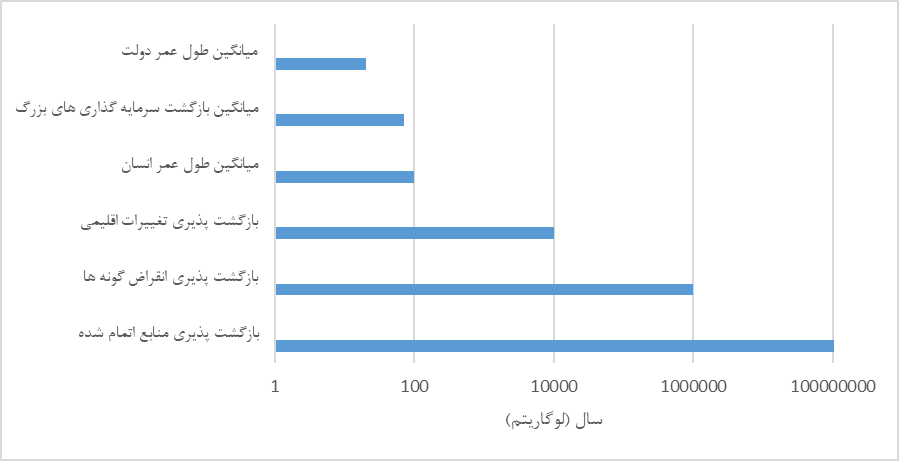
\includegraphics[width=0.9\linewidth]{screenshot001}
	\caption{مقیاس ها برای طبیعت و انسان}
	\label{fig:screenshot001}
\end{figure}
این نمودار بیانگر گستردگی و دامنه آثاری است که نسل امروزی با فعالیت‌های خود بر کره زمین، بر آینده این زیست بوم مشترک بین موجودات زنده می‌گذارد. 

در این گفتار سعی گردیده با توجه به گزارش‌های هیات بین‌الدولی تغییرات‌اقلیمی 
طی سه بند ابتدا به تعریف این پدیده بپردازیم و سپس آثار تغییرات‌اقلیمی را ابتدا بر نظام اقلیم(آثار اولیه) و سپس بر جوامع انسانی(آثار ثانویه) شرح دهیم.









	\subsection*{بند اول: تعریف}\addcontentsline{toc}{subsection}{بند اول: تعریف}
	در این گفتار ابتدا وجوه تماییز تغییرات‌اقلیمی و تغییرات آب‌و‌هوایی مورد بررسی قرار گرفته و سپس با شرح علل این تغییرات، این مفهوم را تعریف نموده‌ایم.


		\subsubsection*{ اول: تغییرات‌اقلیمی یا آب‌و‌هوایی}\addcontentsline{toc}{subsubsection}{ اول: تغییرات‌اقلیمی یا آب‌و‌هوایی}
		میان این دو، اگر چه در ادبیات حقوقی گاها به جای یکدیگر بکار برده می‌شوند، تفاوت وجود دارد. تغییرات آب‌و‌هوایی\LTRfootnote{Weather change.} به رشته‌ای از تغییرات گفته می‌شود که بر سردی و گرمی هوا، کمی و زیادی برف و باران، شدت و ضعف طوفان‌ها و گرد‌باد‌ها در طول چند روز و چند هفته تاثیر می‌گذارد. دانش هواشناسی به پیش بینی آنچه در کوتاه مدت در جو زمین اتفاق می‌افتد، می‌پردازد. 
		
		وقتی از تغییرات‌اقلیمی\LTRfootnote{Climate Change.} صحبت می‌کنیم، تغییراتی مد نظرمان می‌باشد که در بازه طولانی الگو و میانگین آب و هوای روزانه را متاثر می‌کند. امروزه، کودکان مدام روایت‌هایی از پدران و مادران‌شان می‌شنوند که گویای بارش چند متری برف و گاها تونل زدن زیر مسیر‌های برفی و تعطیلی چند روزه مدارسشان در گذشته می‌باشد. در اکثر مناطق کشور کودکان دیگر امکان دریافت چنین تجربه‌هایی را ندارند. این تغییر الگوی بارش برف به خوبی گویای اقلیم تغییر یافته از زمانی که والدین‌شان جوان بودند، می‌باشد.\LTRfootnote{Weather or Climate change, 09-2017, Retrieved from: www.climate.nasa.gov.} 
		
		اگر تابستان‌ها گرمتر از گذشته به نظر می‌رسند و یا وقتی می‌شنویم که مردم در نقاط مختلف جهان ادعا می‌کنند که بهار زودتر از سی سال گذشته رخ می‌دهد. در می‌یابیم که در الگو و نظم اقلیم جهانی تغییراتی بوجود آمده است.
		
		آب و هوا در واقع، شیوه رفتار اتمسفر است با در نظر گرفتن تاثیری که بر زندگی و فعالیت‌های انسان دارد. تفاوت آب و هوا با اقلیم در این است که آب و هوا شامل تغییرات کوتاه ( چند دقیقه تا چند ماه) در اتمسفر است. اقلیم اما میانگین وضعیت آب و هواست در بازه طولانی زمان و فضا. اقلیم آن چیزی است که ما انتظارش را داریم مانند یک تابستان گرم، اما آب و هوا وضعیتی می‌باشد که دریافت می‌کنیم.\LTRfootnote{Roda, Verheyen, \textbf{Climate Change Damage and International Law Prevention Duties and State Responsibility}, Martinus Nijhoff Publishers, 2005, p. 12-13}  















		\subsubsection*{ دوم: تغییرات‌اقلیمی و علل آن}\addcontentsline{toc}{subsubsection}{ دوم: تغییرات‌اقلیمی و علل آن}
		دمای کره زمین وابسته به میزان ورود و خروج انرژی به نظام زمین است. هنگامی که انرژی خورشید جذب زمین می‌شود، زمین گرم گردیده و هنگامی که این انرژی توسط زمین به فضا منعکس می‌شود، زمین شروع به سرد شدن می‌کند. عوامل متعدد طبیعی و انسانی در ایجاد تغییر در چرخه توازن انرژی کره زمین ایفای نقش می‌کنند که شامل: 1- اختلاف میزان انرژی خورشید، 2- تغییرات در میزان انعکاس انرژی وارد شده، از زمین به فضا و 3- تغییرات در اثر‌گلخانه‌ای، که بر میزان گرما کره زمین تاثیر می‌گذارد. این عوامل باعث تغییرات در اقلیم به صورت متعدد می‌شوند.\LTRfootnote{«Causes of Climate Change», 06-2017, Retrieved from: www.archive.epa.gov.}
		اقلیم دارای نظامی پویا و در حال تحول و تغییر بوده، که در تاریخ زمین قابل مشاهده است. این تغییرات که موقت یا با بازه زمانی طولانی و در یک نقطه یا در تمامی سطح کره مسکون رخ می‌دهند، در سه دسته قابل تقسیم بندی می‌باشند. این سه دسته عبارتند از: 1- پروسه‌های طبیعی داخلی 2- تاثیرات انسانی و 3- فشار.
		
		تغییرات ایجاد شده بوسیله فشار در نظام اقلیم، می‌تواند هواویز‌های منتشر شده از سنگ‌های آتشفشانی بوده باشد، یا اینکه بدون فشار خارجی و  به عنوان نمونه در اثر پدیده ال‌نینو باشد. برای مشخص شدن حدود این متن لازم است تمایز قائل شویم میان تغییرات طبیعی اقلیمی، و تغییراتی که در اقلیم بوسیله انسان ایجاد می‌گردد. کنوانسیون چارچوبی تغییرات‌اقلیمی سازمان ملل متحد،\LTRfootnote{United Nations Framework Convention on Climate Change (UNFCCC)} تغییرات‌اقلیمی را به شرح زیر تعریف نموده است: «تغییرات‌اقلیمی به تغییراتی که مستقیما یا با واسطه توسط فعالیت‌های انسان در اقلیم ایجاد گردیده و نسبت اجزای سازنده اتمسفر جهانی را دگرگون می‌نماید گفته می‌شود.»
		
		این تغییرات افزون بر تغییرات‌اقلیمی ایجاد شده بواسطه طبیعت می‌باشد و قابل ارزیابی در بازه زمانی مشخص است. گاهی اوقات به این پدیده تغییرات‌اقلیمی انسان‌آورد گفته می‌شود، تا به خوبی تمایز تغییرات‌اقلیمی طبیعی و انسانی را بیان کند. اشاره به چنین تفاوتی از این باب حائز اهمیت می‌باشد که الزامات حقوقی و مسئولیت را صرفا به انسان می‌توان اختصاص داد. برای این منظور باید تاثیر انسان بر پدیده تغییرات اقلیم را در پس‌زمینه آثار طبیعت بر این پدیده شناسایی نمود.\LTRfootnote{Ibid., p. 13-17.}  
		
		اكسیژن، نیتروژن، و آرگن روی هم رفته 96/99 درصد از جو را تشكیل مى دهند. این گازها در سرمایش و گرمایش زمین نقش زیادى ندارند. 4/0 دهم درصد باقى مانده را، به ترتیب اهمیت، كربن دى اكسید، متان، نیتروزاكسید، ازن، و كلروفلوروكربن‌ها تشكیل مى دهند. این گازها، تابش خورشید را از بالاى جو به پایین راه مى دهند، ولى مانع خارج شدن تابشِ میكرومترىِ زمین به فضا می‌شوند. این گازها، نقشى مانند شیشه در دیوارها و سقف گل خانه دارند و به همین سبب به گازهاى گلخانه اى معروف‌اند. اگر مقدار این گازها در جو بالا رود، زمین گرم می‌شود.\RTLfootnote{ ثبوتی، یوسف، «اقلیم و تغییرات آن در سده‌های بیستم و بیست و یکم»، فصلنامه نشاء علم، سال اول، شماره 2، خرداد 1390، ص. 9-10.}
		
		كربن دى اكسید، بیشتر از سوختن سوخت‌هاى فسیلى و غیرفسیلى، از دم و بازدم موجودهاى زنده، از تبدیل سنگ‌هاى كربن دار به تركیب‌هاى سیلیسى در طبیعت و در صنعت سیمان نشر مى شود. از سوى دیگر، كربن دى اكسید به وسیله روییدنى‌ها، مرجان‌ها و موجودهاى دریایىِ صدف دار جذب مى شود و در آب اقیانوس‌ها به خوبى حل مى شود. متان، بیشتر از تجزیه تركیب‌هاى آلى گیاهى و حیوانى در مرداب‌ها، كف دریاها و جنگل‌ها و نشخوار نشخواركننده‌ها منتشر می‌شود. نیتروزاكسید در طبیعت بوجود مى‌آید و از بین مى‌رود. مصرف روزافزون سوخت‌هاى فسیلى و كودهاى شیمیایى به افزایش آن در جو كمك مى‌كند. ازن در لایه‌هاى بالاى جو در اثر تابش فرابنفش خورشید بوجود مى‌آید و اثر خنك كنندگى دارد. ولى، در لایه‌هاى پایین جو و سطح زمین، ازن در انجام فرآیندهاى صنعتى، مانند جوشكارى و جرقه‌هاى الكتریكى تولید مى‌شود و گرم کننده جو و زمین است. كلروفلوروكربن‌ها به طور طبیعى به وجود نمى‌آیند. انسان ساخت هستند و در افشانه‌ها و ماشین‌هاى سرمازا به‌ كار می‌روند. پیمان نامه‌هاى بین‌المللى،\RTLfootnote{در سال ۱۹۸۵ کنوانسیون وین برای حفاظت از لایه ازن توسط سازمان ملل متحد و دیگر کشورها تدوین شد و سپس در سال ۱۹۸۷ پروتکل مونترال در سازمان ملل متحد توسط ۴۶ کشور پذیرفته شد.} تولید انواع آسیب رسان آنها را محدود كرده است.\LTRfootnote{Intergovernmental Panel on Climate Change (IPCC), 2007, «The Physical Science Basis», Cambridge University Press.}
		
		
		بیش از 20 درصد از کربن دی اکسید اضافه شده در جو به مدت بیش از 1000 سال باقی می‌ماند. انتشار سالانه کربن دی اکسید از سوخت‌های فسیلی و تولید سیمان در سال 2011 به میزان 9.5 گرم بوده است که 54 درصد بالاتر از سطح 1990 می‌باشد. در جهان، انتشار گازهای گلخانهای از سال 1970 به حدود 75 درصد افزایش یافته است.
		















	\subsection*{بند دوم: تاثیرات تغییرات‌اقلیمی  بر نظام اقلیم}\addcontentsline{toc}{subsection}{بند دوم: تاثیرات تغییرات‌اقلیمی  بر نظام اقلیم}
	
	
	
	مشاهدات نظام اقلیم مبتنی بر‌اندازه گیری‌های مستقیم و سنجش از راه دور از ماهواره‌ها و دیگر نظام عامل‌ها است. مشاهدات جهانی در مقیاس وسیع در اواسط قرن نوزدهم برای دما و سایر متغیرها آغاز شد و مجموعه‌های گسترده تر و متنوعی از مشاهدات در دسترس برای دوره 1950 به بعد وجود داشت. تجدید ساختارهای آب‌و‌هوایی که در یک زمان خاص در گذشته زمین‌شناسی شایع است حکایت از برخی از رکورد‌ها دارد که صدها تا میلیون‌ها سال پیش وجود داشته است. با هم، آنها دیدگاه جامع از تغییرات و تغییرات درازمدت در جو، اقیانوس، کریوسفر و سطح زمین را ارائه می‌دهند.\LTRfootnote{Intergovernmental Panel on Climate Change 2013 (IPCC), The Physical Science Basis, Cambridge University Press, p. 4.}
	
	گرم شدن نظام اقلیم که از دهه 1950 شروع شده است در طول دهه‌ها تا هزاران سال پیش بی سابقه بوده است. جو و اقیانوس گرم شده‌اند، میزان برف و یخ کاهش یافته است، سطح دریا و غلظت گازهای گلخانهای افزایش یافته است.
	
	
	
	
	
	\begin{enumerate}
		
		
		
		
		
		
		
		
		\item  جو\\
		هرکدام از آخرین سه دهه در سطح زمین به طور پیوسته گرمتر از سال‌های 1850 بوده است . در نیمکره شمالی، سالهای 2012-1983، احتمالا گرمترین دوره 30 ساله 1400 سال گذشته بود. دمای ترکیبی سطح اقیانوس و  زمین در سطح جهانی و داده‌هایی که به وسیله یک روند خطی محاسبه شده است، در طول دوره زمانی 1880 تا 2012، گرم شدن $ 0.85 $ درجه سانتیگراد را نشان می‌دهد. افزایش کلی دما بین میانگین 1900-1850 و دوره 2012-2003، $ 0.78 $ درجه سانتیگراد است، که مبتنی بر طولانی ترین داده‌های موجود در دسترس است. وقتی محاسبه آمار منطقهای به‌ اندازه  کافی انجام شد، تقریبا تمام سطح زمین گرما را تجربه نموده بودند. تقریبا مطمئن هستیم که گشت کره\LTRfootnote{Troposphere.}  (صفر تا 10 کیلومتری زمین) از اواسط قرن بیستم میلادی گرم گشته است. افزایش روز‌ها و شب‌های گرم و کاهش روز‌ها و شب‌های سرد در سطح جهانی بسیار محتمل است.\LTRfootnote{Ibid, p. 5-7.}
		
		
		
		
		
		
		
		
		
		
		
		
		
		
		
		
		\item	 اقیانوس\\
		تقریبا مطمئن هستیم که بخش بالایی اقیانوس\LTRfootnote{Upper Ocean.} (700-0 متر) از سال 1971 تا 2010 گرم شده است. در مقیاس جهانی، نزدیکترین سطح آب(75 متر)، در سال‌های 1971 تا 2010 با 11/0 درجه سانتیگراد در هر دهه گرم گردیده است. بیش از 60 درصد از انرژی خالص در نظام اقلیمی در اقیانوس بالا در طی نمونه دوره نسبتا خوب 40 ساله از سال 1971 تا 2010 ذخیره گردیده و حدود 30 درصد در بخش زیرین اقیانوس (زیر 700 متر) ذخیره می‌شود. افزاش دما در بخش بالایی اقیانوس در این دوره پیش بینی می‌شود. احتمال زیادی وجود دارد که از سال 1950 در مناطقی با تبخیر بالا شوری غالب باشد، و در مناطقی با بارش زیاد شوری کمتر گردد. این آمار منطقهای به صورت غیر مستقیم بیانگر این نکته می‌باشد که روند تبخیر و بارندگی در اقیانوس‌ها تغییر نموده است.\LTRfootnote{Ibid, P. 8.}
		
		
		
		
		
		
		
		
		
		
		
		
		
		
		
		
		
		
		
		\item  سرماکره\RTLfootnote{سرماکره (Cryosphere)، برف و یخ یخپال‌های کوهستانی و قطب ها و زمین‌های یخ زده را شامل می‌شود.}\\
		در طول دو دهه گذشته، ورقه‌های یخ گرینلند و قطب جنوب، بشدت کاهش یافته‌اند. یخچال‌ها تقریبا در سراسر جهان در حال کاهش بوده‌اند. و پوشش برف بهار و یخ دریای قطب شمال در نیمکره شمالی همچنان در حال کاهش می‌باشد. میانگین افت یخ در یخچال‌های طبیعی در سراسر جهان، به استثنای یخچال‌های طبیعی در حاشیه یخچال‌های یخ، احتمالا 226 میلیون تن\RTLfootnote{افت 100 میلیون تن یخ در سال، معادل 28/0 میلیمتر افزایش سطح آب دریا می‌باشد.}  در سال‌های 1971 تا 2009 می‌باشد. 
		
		صفحات یخ گرینلند و قطب جنوب، بزرگترین اجرام یخ در جهان هستند و در نظام اقلیمی جهانی، نقش مهمی ایفا می‌کنند. هر دو ورقه یخ از سال 1992 مقدار زیادی از یخ را از دست داده‌اند. افت یخ تجمعی از گرینلند از سال 1992 تا 2015 به 3600 گیگاتن رسید و موجب افزایش سطح جهانی آب دریا در حدود 10 میلیمتر شد. شکل مربوطه برای قطب جنوب 1500 گیگاتن است که مربوط به حدود 5 میلیمتر افزایش سطح جهانی آب دریا از سال 1992 است. پیش بینی‌های مدل کاهش بیشتر یخ قطبی در آینده را نشان می‌دهد، اما این موضوع همراه با یک عدم اطمینان بزرگ است. برابر تخمین‌ها ذوب ورقه‌های یخ قطبی تا 50 سانتی متر افزایش سطح دریا در طول قرن 21 را در پیش خواهد داشت. پیش بینی‌های بسیار طولانی مدت (تا سال 3000) نشان دهنده افزایش چند متری سطح دریا، با ذوب شدن ورقه‌های یخ است.\LTRfootnote{Greenland and Antarctic ice sheets, 20 Dec 2016, Key messages, Retrieved from: www.eea.europa.eu, 05/09/18.}
		
		میزان پوشش برف نیمکره شمالی از اواسط قرن بیستم کاهش یافته است. میزان بارش برف نیمکره شمالی در ماه مارس و آوریل به میزان 1.6 درصد و در ماه ژوئن 11.7 درصد در هر دهه در طول دوره 1967 تا 2012 کاهش یافت. در طول این دوره، میزان پوشش برف در نیمکره شمالی در هر ماه افزایش قابل ملاحظهای نشان نداد. با اطمینان بالایی میتوان ادعا نمود که از اوایل دهه 1980 دمای هوا در سراسر جهان افزایش یافته است. گرم شدن مشاهده شده در مناطق آلاسکا شمالی به 3 درجه سانتیگراد (اوایل 1980 تا اواسط سال 2000) و در قسمت شمالی اروپایی روسیه تا 2 درجه سانتیگراد (1971 تا 2010) بود. در منطقه دوم، در طول دوره 1975 تا 2005، کاهش قابل توجهی در ضخامت مرجان و رسوبات مشاهده شده است.\LTRfootnote{Intergovernmental Panel on Climate Change 2013 (IPCC), Op.cit., P. 9.}
		
		
		
		
		
		
		
		\item  سطح دریا\LTRfootnote{Sea Level.}\\
		هیات بین‌المللی تغییرات‌اقلیمی با سطح بالایی از اطمینان، افزایش سطح آب دریا از اواسط قرن 19 نسبت به سطح آن در دو هزاره قبلی را تایید می‌کند. سطح آب دریا از 1901 تا 2010، چیزی حدود 19/0 میلیمتر افزایش یافته است. اطلاعاتی که از سطح دریا با گذر از قرن 19 و در ابتدای قرن 20 وجود دارد بیانگر این امر است که سطح آب دریا از کم به زیاد طی دو هزاره گذشته افزایش یافته است. 
		
		از اوایل دهه 1970، افت انبوه جرم یخچال و انبساط دمایی اقیانوس، که ناشی از گرمایش جهانی می‌باشد، حدود 75 درصد از افزایش سطح جهانی دریا را توضیح می‌دهد. در طول سالهای 1993 تا 2010، افزایش جهانی سطح دریا در مقایسه با مجموع سهم مشاهده شده از انبساط دمایی اقیانوس به علت گرم شدن1/1 میلیمتر در سال، از تغییرات یخچالهای طبیعی76/0 میلیمتر در سال، صفحات یخ گرینلند 33/0 میلیمتر در سال، ورق یخ قطب جنوب27/0 میلیمتر در سال و ذخیره آب زمین38/0 میلیمتر در سال بوده است، که مجموع این سهم‌ها عبارتند از 8/2 میلیمتر در سال. با اطمینان بالایی دریافته‌ایم که حداکثر میانگین جهانی سطح دریا در طول آخرین دوره بین‌یخبندانی، (116000 تا 129000 سال پیش) برای چندین هزار سال، حداقل و حداکثر به ترتیب 5 و 10 متر بالاتر از حال حاضر بوده است.\LTRfootnote{Ibid, P. 11.}
		همچنین علت دیگر افزایش سطح آبها این است که با گرم شدن اقیانوس ها، آب منبسط شده و سطح گسترده تری را پوشش می‌دهد.\LTRfootnote{Islands disappear under rising seas, 4 november 2018, Retrieved from: news.bbc.co.uk, (14 june 1999).}
		
		سطح آب های دریا انتظار می‌رود که در سال 2100 با درجه گرمای 5/1 سانتی گراد کره زمین چیزی حدود 1/0 متر کاهش یابد. سطح آب ها حتی بعد از سال 2100 به افزایش خود ادامه خواهد داد. اندازه و نرخ رشد سطح آبها به میزان کاهش یا افزایش انتشار گاز های گلخانهای توسط نسل امروز و نسل های آینده وابسته می‌باشد. بدیهی است نرخ رشد پایین تر سطح آبها فرصت های بسیاری را برای انطباق با شرایط جدید به انسان می‌دهد.\LTRfootnote{Intergovernmental Panel on Climate Change(IPCC), «Summary for Policymakers», 2018, P. 9.}
		
		
		
		
		
		
		
		
		
		
		\item کربن و دیگر چرخه های زیست گیاه شناسی\LTRfootnote{Carbon and Other Biogeochemical Cycles.}
		
		غلظت اتمسفر از دی اکسید کربن، متان و اکسید نیتروژن به سطح بی سابقه ای، در حداقل 800000 سال گذشته افزایش یافته است. غلظت دی اکسید کربن از زمان‌های قبل از صنعتی‌شدن 40درصد  افزایش یافته است، که این میزان در درجه اول ناشی از انتشار سوخت‌های فسیلی و درجه دوم از تولید گازهای گلخانهای ناشی از تغییر کاربری اراضی خالص می‌باشد. اقیانوس حدود 30‌درصد از دی اکسید کربن تولید شده انسانی را جذب کرده است، رخدادی که منجر به اسیدی شدن اقیانوس می‌شود.
		
		غلظت گاز‌های گلخانهای همچون کربن‌دی‌اکسید، متان و اکسید‌نیتروژن، از زمان 1750 به علت فعالیت‌های انسانی افزایش یافته است. در سال 2011، غلظت این گاز‌ها، به ترتیب 391 بخش در میلیون، 1803 و 324 بخش در میلیارد بود، که حدودا 40، 150 و 20 درصد بیشتر از مقادیر دوره پیشاصنعتی می‌باشد. غلظت کربن‌دی‌اکسید، متان و اکسید‌نیتروژن، در حال حاضر به طور قابل ملاحظهای بیش از بالاترین غلظت ثبت شده در هسته یخ طی 800000 سال گذشته است.متوسط افزایش غلظت این گاز‌ها در جو در طی قرن گذشته، در 22000 سال گذشته بی‌سابقه بوده است.
		
		اسیدی شدن اقیانوسها با کاهش 
		\LTRfootnote{potential of hydrogen PH \persian(یک کمیت لگاریتمی است که میزان اسیدی یا بازی بودن مواد را مشخص می‌کند.)}
		PH مشخص می‌گردد. pH آبهای سطحی اقیانوس از زمان آغاز عصر صنعتی 1/0 درصد کاهش یافته است، که مربوط به افزایش 26 درصدی غلظت یون هیدروژن است.\LTRfootnote{Ibid, P. 12.}
	\end{enumerate}
	
	
	
	\subsection*{بند سوم: تاثیرات تغییرات‌اقلیمی بر جوامع انسانی}\addcontentsline{toc}{subsection}{بند سوم: تاثیرات تغییرات‌اقلیمی بر جوامع انسانی}
	
		
		
\begin{enumerate}
	
			\item	تاثیر تغییرات‌اقلیمی بر نیاز‌های اولیه\\
نیاز‌های اولیه مورد اشاره شامل کشاورزی، تامین و کیفیت آب، سلامتی و مسکن می‌باشد، که مورد بررسی واقع می‌شود. 
				\begin{itemize}
					\item کشاورزی و خوراک\\
تغییرات در اقلیم تاثیر بسزائی در تولید مواد غذایی در سراسر کره زمین داشته است. استرس گرما، خشکسالی و سیلاب‌ها منجر به کاهش محصولات زراعی و تولیدات دامی می‌شود. مناطقی از کره که هم اکنون متاثر از خشکسالی می‌باشند مانند استرالیا و بخشی از آفریقا که در جنوب صحرای کبیر قرار دارد، مشکل کمبود آب در دسترس برای آبیاری را تجربه خواهند نمود.

در عرض جغرافیایی متوسط تا بالا پیش بینی می‌شود که رویش محصولات زراعی قَله با توجه به میزان گرمای منطقه و نوع محصول به آرامی افزایش یابد. در عرض‌های جغرافیایی کمتر، محصولات کشاورزی قَله کاهش خواهد یافت. بیشترین کاهش در محصولات قَله در مناطقی با آب و هوای خشک و استوایی رخ خواهد داد. به عنوان نمونه تا سال 2050 پیش بینی می‌شود که در برخی کشور‌های آفریقایی کاشت و برداشت محصول گندم بیش از 35 درصد، کاهش یابد. \LTRfootnote{Intergovernmental Panel on Climate Change 2014 (IPCC), «Impacts, Adaptation, and Vulnerability Part B: Regional Aspects», Cambridge University Press, United States of America, P. 1218.}

تغییرات‌اقلیمی بر صنعت شیلات در عمده مناطق کره زمین تاثیر گذاشته است. افزایش دمای اقیانوس‌ها باعث شده بعضی گونه‌های دریایی به آب‌های خنک تر تغییر مکان دهند. صنعت شیلات به جهت تامین خوراک و اینکه اقتصاد بسیاری کشور‌ها به آن وابسته می‌باشد، دارای اهمیت است. به عنوان نمونه، خوراک بیش از 40 میلیون انسان وابسته به نوعی ماهی می‌باشد که از دلتای مکونگ\RTLfootnote{ین رود بزرگترین رود آب شیرین برای ماهی گیری در جهان می‌باشد که از تبت سرچشمه گرفته و از چین و هندوچین می‌گذرد و به دریای جنوب چین می‌ریزد} در آسیا، تامین می‌گردد. پیش بینی می‌شود، کاهش جریان آب و افزایش سطح آب دریاها، برکیفیت آب و گونه‌های ماهی در مناطقی مانند نمونه بالا تاثیر منفی خواهد گذاشت، و این عامل بر تامین مواد غذایی جوامعی که به این گونه منابع وابسته می‌باشند، تاثیر خواهد داشت.\LTRfootnote{ Intergovernmental Panel on Climate Change (IPCC) 2014, Op.cit., P. 1355.}

				تغییرات‌اقلیمی امنیت غذایی را در ابعاد جهانی منطقهای و محلی بوسیله اختلال در دسترسی به خوراک، کاهش دستیابی به منابع غذایی و سخت کردن بهره‌برداری تحت تاثیر قرار می‌دهد. ریسک اقلیم در امنیت غذایی برای جمعیت فقیر و مناطق گرمسیری بسیار زیاد می‌باشد.
				\LTRfootnote{International Climate Impact, 06-2017,  Retrieved from: 19january2017snapshot.epa.gov} \\
					\item تامین و کیفیت آب\\
مناطق خشک و نسبتا کم آب مانند منطقه مدیترانه، جنوب آفریقا، و شمال برزیل مستعد تاثیرات تغییرات‌اقلیمی بر تامین آب می‌باشند. در قرن آینده این مناطق، مخصوصا بخش‌هایی که به علت خشکسالی، فشار جمعیت، و بهره‌برداری بی‌رویه منابع آبی، زنگ خطر کم آبی کاهش منابع آبی را تجربه خواهند کرد.

در اثر تغییرات‌اقلیمی، آب در مناطق بسیاری، در حال تبدیل شدن به یک منبع کمیاب است، در حالی که در برخی دیگر مناطق، آب کافی وجود خواهد داشت. دسترسی به آب به میزان بسیاری منوط به میزان بارش نزولات آسمانی و روان آب‌ها می‌باشد. با افزایش 2.7 فارنهایت در دمای جهان میانگین بارش سالانه پیش بینی می‌شود بین 10-50 درصد در عرض جغرافیایی بالا و در برخی مناطق گرمسیری افزایش یابد و در همین حین در مناطق خشک و عرض‌های جغرافیایی متوسط و نیمه حاره همین حدود کاهش یابد.\LTRfootnote{Intergovernmental Panel on Climate Change (IPCC) 2013, Op.cit., P. 91.} با افزایش دما بارش برف در بسیاری مناطق کاهش می‌یابد. یخچال‌های قطب با سرعت بی سابقهای آب می‌شوند و دسترسی به آب را در مناطقی که وابسته به آب شیرین یخچال‌ها در بهار و تابستان هستند محدود می‌سازد. خشکسالی مدام گسترش می‌یابد. افزایش بارش، سطح منابع آب آشامیدنی را افزایش نمی‌دهد بلکه باعث افزایش سیل‌ها می‌شود.

کیفیت آب برای بوم‌سازگان، بهداشت و سلامت بشر، کشاورزی و دیگر اهداف حائز اهمیت است. افزایش دما، تغییر در بارش، افزایش سطح آب و حوادث طبیعی از جمله عوامل تاثیر گذار بر کیفیت آب می‌باشند. طوفان‌های بارانی بسیار بزرگ باعث ورود منابع آلوده کننده به رودخانه‌ها شده و آب زیادی ممکن است نظام فاضلاب و ضربه‌گیر‌های طبیعی را درهم بشکند. افزایش آلودگی مانند افزایش دمای آب می‌تواند عامل افزایش انفجاری رشد جلبک و خزه و افزایش بالقوه باکتری در مجموعه آب شود. در مناطق ساحلی و جزایر کوچک، آب شور ناشی از افزایش سطح آب دریا و موج‌های طوفان امکانات آبی را تهدید می‌کند. این آثار جوامع را ملزم می‌کند تا بدنبال منابع آبی مطمئن برای استفاده بشر باشد.\LTRfootnote{Intergovernmental Panel on Climate Change (IPCC) 2014, Op.cit., PP. 229-269.}
					\item سلامت بشر\\
ریسک بیماری‌ های ناشی از تغییرات‌ اقلیمی در کشور‌هایی که امکانات مناسبی جهت مقابله با بیماری را ندارند بسیار بیشتر می‌باشد. نمونه‌های بسیاری از بیماری‌های مرتبط با تغییرات‌اقلیمی وجود دارد. افزایش دمای کره با استرس گرما به صورت جدی لینک شده است. بدتر شدن کیفیت هوا که معمولا همراه با موج گرما و حریق‌های گسترده رخ می‌دهد منجر به مشکلات تنفسی و تشدید آن و بیماری‌های قلبی می‌شود.\LTRfootnote{Ibid, P. 1057.} اثر تغییرات‌اقلیمی بر کشاورزی و نظام غذایی می‌تواند باعث افزایش نرخ سوتغذیه و بیماری‌های مرتبط با غذای کم کیفیت شود. 

تغییرات‌اقلیمی می‌تواند بر بیماری‌های واگیردار موثر باشد. گسترش بیماری همه‌گیر مننژیت عموما با تغییرات‌اقلیمی مخصوصا خشکسالی لینک شده است. مناطقی در زیر صحرای آفریقا و آفریقای غربی به گسترش مننژیت حساس بوده و به صورت خاص در ریسک می‌باشد اگر خشکسالی گسترش یافته و شدید شود. احتمال گسترش بیماری‌های قابل حمل به وسیله پشه مانند مالاریا، تب استخوان شکن و ویروس غرب نیل  در مناطقی که پیش بینی می‌شود بارش و سیل بیشتری را دریافت می‌کنند وجود دارد. افزایش باران و دما منجر به گسترش بیماری تب استخوان شکن می‌باشد.\LTRfootnote{Ibid, P. 722.} 

تغییر در الگوی بارش و حوادث حاد اقلیمی منجر به کاهش آثار سلامت می‌شود به خصوص هنگامی که قدرت، آب یا نظام حمل و نقل مختل گردد. بیماری اسهال که ناشی از آب آلوده و منابع غذایی می‌باشد به یک نگرانی بزرگ به خصوص برای کودکان تبدیل می‌گردد. اثر تغییرات‌اقلیمی بر سلامت روانی و رفاه، بخش جدایی ناپذیر از مجموعه اثار مرتبط با تغییرات‌اقلیمی بر سلامت بشر می‌باشد. آثار تغییرات‌اقلیمی بر سلامت روانی طیفی از استرس ‌اندک و نشانه‌های اضطرار تا اختلالات بالینی مثل اضطراب، افسردگی، اختلال فشار روانی و افکار خودکشی را شامل می‌شود.\LTRfootnote{Ibid, P. 732.} 

گروه‌های خاصی از مردم در کشور‌های کم درآمد به صورت خاص در معرض آثار معکوس تغییرات‌اقلیمی در سلامت هستند. این گروهای در ریسک شامل مردم فقیری که در شهر زندگی می‌‌کنند، گروه بزرگسالان، کودکان، جوامع سنتی، کشاورزان و جمعیت ساحلی می‌باشند. بسیاری از مناطق مانند اروپا، آسیای جنوبی، استرالیا و شمال آمریکا اثرات بهداشتی مرتبط با گرما را تجربه کرده‌اند. جمعیت روستایی، بزرگسالان، کارگران بیرون خانه و آنهایی که دسترسی به تهویه مطبوع ندارند، بیشتر از دیگران مستعد بیماری و مرگ و میر مرتبط با گرما می‌‌باشند.
					\item مسکن\\
تغییرات‌اقلیمی بر مهاجرت افراد در داخل و بین کشور‌های جهان، تاثیر می‌گذارد. عوامل بسیار زیادی به مهاجرت افراد به مناطق دیگر اثر می‌گذارد. این عوامل می‌تواند شامل اختلافات بر سر منابع، افت خدمات بوم‌سازگان، کمبود زمین کشاورزی بادوام یا آب تازه، و رویداد‌های شدید مانند سیل، خشکسالی و طوفان باشد.\LTRfootnote{Ibid, P. 1353.} 

رویداد‌های شدید، بسیاری از مردم را مخصوصا در مکان‌هایی که مردم توانایی یا منابع برای پاسخ‌گویی و بازسازی پس از فاجعه را ندارند، بی خانمان می‌کند. مدل‌های مختلفی از این قبیل رویداد‌ها، که اختلافات موجود را تشدید می‌کند، به صورت مکرر و شدید در حال رخ دادن است. این خود موجب افزایش میزان مهاجرت‌ها، حین و پس از این رخداد‌ها می‌شود. 

شهرک‌های ساحلی و نواحلی کم ارتفاع به ویژه در برابر تاثیرات تغییرات‌اقلیمی مانند افزایش سطح آب، فرسایش، و طوفان‌های شدید، آسیب پذیر می‌باشند. افزایش دمای اقیانوس و اسیدی شدن آن، همچنین عامل تهدید بوم‌سازگان ساحلی می‌باشد. با نابود شدن زیستگاه‌های ساحلی (مانند جزایر سنگی، تالاب‌ها، دلتا‌ها و مصب‌ها) سکونت‌گاه‌های ساحلی بیشتر در معرض سیل ناشی از طوفان‌های شدید و فرسایش قرار می‌گیرند. هم کشور‌های توسعه یافته و هم در حال توسعه در معرض اثرات افزایش سطح آب می‌باشند.\LTRfootnote{Ibid, P. 381.} 
				\end{itemize}
			\item 	جمعیت آسیب‌پذیر	\\
گروه‌های بومی در مناطق مختلف مانند آمریکا، آمریکای جنوبی و لاتین، اروپا و آفریقا، در حال تجربه تهدیدات مربوط به زندگی سنتی هستند. زندگی بومیانی که در جزایر کم سطح سکنی گزیده‌اند توسط افزایش سطح آب و رویداد‌های شدید تهدید می‌شود. افزایش دما، و کاهش برف، یخ و لایه همیشه یخ بسته زمین گروه‌هایی را که در کوهستان و مناطق قطبی زندگی می‌کنند تهدید می‌کند. تغییرات‌اقلیمی در این مناطق بر شکار، صید، حمل و نقل و دیگر فعالیت‌ها تاثیر می‌گذارد.

تقریبا 4/1 میلیارد انسان، که شامل 5/1 جمعیت کره زمین می‌شود زیر معیار‌های بانک جهانی در مورد فقر و در فقر شدید زندگی می‌کنند. گروه‌های کم درآمد بسیاری وابسته به خدمات و منابع عمومی مانند آب، انرژی و حمل و نقل هستند. حوادث شدید این منابع و خدمات را مختل می‌کند. بسیاری از مردم در کشور‌های کم درآمد امکان دستیابی به مکانیزم‌های انطباق پذیری مانند تهویه مطبوع، گرما یا بیمه حوادث را ندارند. این کمبود ظریفت انطباق پذیری، جمعیت ضعیف زمین را در برابر رویداد‌های شدید اقلیمی آسیب پذیر نموده و با منجر شدن به فقر بیشتر و تثبیت آن، وضعیت این گروه‌ها را تشدید می‌کند. 

بزرگسالان و کودکان نسبت به آثار تغییرات‌اقلیمی همچنین گروه حساس می‌باشند. نظام تنفسی،‌ ایمنی و عصبی در حال توسعه کودکان آنها را نسبت به برخی آثار تغییرات‌اقلیمی همچون حوادث متعاقب و شدید، افزایش گرما و آلودگی شدید هوا بیشتر حساس می‌کند. جمعیت بزرگسال همچنین با توجه به نحیف بودن و تغییر پذیری ‌اندک، در ریسک هستند. گرمای شدید و طوفان می‌تواند به صورت نامتناسب بر گروه بزرگسالان تاثیر بگذارد.\LTRfootnote{Ibid, P. 717-718.} 

تاثیر تغییرات‌اقلیمی با توجه به جنسیت می‌تواند متفاوت باشد. زنان نرخ مرگ و میر بیشتری در اثر طوفان‌ها و رویداد‌های شدید  به نسبت مردان دارند، اگرچه تنوع منطقهای در آمار وجود دارد. در برخی نقاط مردان در سن کاری که خارج از خانه مشغول می‌باشند بیشتر در برابر مرگ و میر ناشی از گرما آسیب پذیر هستند. زنان در کشور‌های در حال توسعه در برابر حوادث شدید با توجه به تفاوت‌های جسمی و میزان فقر و بارداری یا نرسیدن خوراک کافی به بدن گروه آسیب پذیر محسوب می‌شوند.\LTRfootnote{Ibid, P. 635.}
			
			
			
			
			
			
			
			
			
			
			\item 	امنیت ملی	\\
امنیت انسان بستگی به وجود یک نظام دارد که در آن هر فرد عقلانی برابر محاسباتش به این نتیجه برسد که همکاری با نظام بیشتر از شورش، جنگ داخلی، تروریسم، جرم و غیره سود آور است. افراد عقلانی اگر رفاه و امنیت فردی و رونق و امنیت آینده خود را در همکاری با نظام تضمین شده بیابند، به این فعالیت ها اقدام نخواهند کرد. بنابراین، یک نظام امن باید بتواند استاندارد قابل قبول زندگی و وعده یک آینده ی پایدار برای هر فرد را تضمین کند.\LTRfootnote{Gough, Mark, «Human Security: The Individual in the Security Question - The Case of Bosnia», Contemporary Security Policy, V. 23, 2002, PP. 154-155.}

با توجه به تفاوت در تقسیم منابع در سطح کره زمین، تغییرات‌اقلیمی به شیوه های متفاوتی بر امنیت انسانی تاثیر خواهد گذاشت. به عنوان نمونه: خلاف کشورهای صنعتی، که کشاورزی نیازمند یک یا دو درصد از نیروی کار است در کشور‌های شرقی 85 درصد از جمعیت به عنوان اصلی‌ترین منبع درآمد خود به کشاورزی وابسته می‌باشند. اکثر این جمعیت به کشاورزی مشغول هستند به طوری که 46 درصد از مردم روستایی زیر خط فقر و با 55/0 دلار در روز زندگی می‌کنند.\LTRfootnote{Jon Barnett, W. Neil Adger, «Climate change human security and violent conflict», Political Geography, V 26, 2007, P. 641.} 

انتظار می‌رود با افزایش آثار تغییرات‌اقلیمی نگرانی‌ها در خصوص امنیت ملی و آمار درگیری‌های بین‌المللی افزایش یابد. تغییرات‌اقلیمی عامل ناپایداری در کشور‌ها، صدمه در دسترسی به آب و غذا، آسیب دیدن زیرساخت‌ها، شیوع بیماری‌ها، آواره شدن و بی خانمانی گروه بسیاری از مردم می‌باشد.\LTRfootnote{Intergovernmental Panel on Climate Change 2014 (IPCC), Op.cit., P. 733.} 

بسیاری از نگرانی‌ها حول محور منابع طبیعی مانند آب می‌چرخد. در بسیاری از مناطق زمین دسترسی به آب تبدیل به یک معضل محلی و منطقه‌ای شده است. دسترسی به منابع مطمئن آب در این مناطق بسیار با ارزش می‌باشد. تغییرات در میزان و زمان بارش امکان تبدیل شدن محدودیت‌های‌ اندک را به اختلافات آینده ایجاد می‌کند.\LTRfootnote{Ibid, p. 253.}
شواهد نشان می‌دهد بیشترین نزاع ممکن است بین جوامع محلی، گروه‌های اجتماعی-اقتصادی و ایالت/استان‌ها رخ دهد، در حالی که تعاملات دوجانبه و چند جانبه شاهد همکاری رسمی در مورد منابع است.

امنیت غذایی مورد تهدید در برخی بخش‌های آسیا و زیر صحرای آفریقا عامل ایجاد اختلافات می‌باشد. رشد بی رویه جمعیت و تغییرات در میزان بارش و دما در میان دیگر عوامل بر تولید محصولات در حال تاثیر گذاری می‌باشد. نتیجه کمبود مواد غذایی ریسک بحران‌های بشردوستانه و مهاجرت جمعیتی را در مرز‌های ملی افزایش داده و نهایتا یکپارچگی سیاسی کشور‌ها را ناپایدار می‌نماید.

اگر گرم شدن کره زمین بیش از یک آستانه خاص ادامه یابد، که باعث از دست دادن تقریبا کامل یخچال یخ گرینلند در طی یک هزاره یا بیشتر شود، سطح جهانی دریا به صورت متوسط حدود 7 متر افزایش خواهد یافت. آینده تغییرات سطح دریا در حوزه منطقهای متفاوت خواهد بود، اما پیش بینی می‌شود در حدود 70 درصد از خطوط ساحلی، 20 درصد از میانگین جهانی تغییر سطح دریا را تجربه کنند.\LTRfootnote{Ibid, P. 188-189.} از دست دادن مداوم پوشش یخ در قطب اقیانوس اطلس، همراه با پیامد‌های امنیت ملی می‌باشد. اقیانوس اطلس دارای تاریخچهای طولانی از فعالیت نسبتا کم کشتی رانی اگرچه در حال رشد دارد که شامل مسیر‌های حمل و نقل دریایی قطب شمال می‌شود. 

کاهش پوشش یخ دریا به رشد فعالیت‌های دریانوردی می‌انجامد. مسیر شمال-غرب بواسطه تغییرات‌اقلیمی بین آسیا و اروپا برای اولین بار در سال 2007 خالی از پوشش برف گردید.\LTRfootnote{Michael Byers, Suzanne Lalonde, «Who owns the Northwest Passage?», Journal of Transnational Law, v. 42, 2009, P. 1138.}اگر چه شمار زیادی از عوامل بین‌المللی دیگر بر پتانسیل رشد دریانوردی تاثیر می‌گذارد. در مورد اقیانوس قطب شمال، افزایش دریانوردی به معنای اهمیت دوچندان مباحثی همچون حاکمیت (اولویت در کنترل یک منطقه)، امنیت (مسئولیت نظارت بر مسیر‌ها)، حفاظت  محیط‌زیست دریایی (کنترل آلودگی هوا و آبراه کشتی، سرو صدا، صدمه کشتی به وال‌ها) و ایمنی (مسئولیت نجات و پاسخ) می‌باشد.\LTRfootnote{Arctic Council, Arctic Marine Shipping Assessment Report, 2009, Retrieved from: www.pmel.noaa.gov, 9/9/2018, P. 5.} 

همچنین پس از بررسی دانشمندان رابطه میان تاثیر تغییرات‌اقلیمی و ایجاد زلزله بررسی شد. در این بررسی دکتر برندس\LTRfootnote{Brandes.} به همراه تیم خود، بررسی نمودند که آیا آب شدن یخچال های قطب بر تغییر شکل یک منطقه از دانمارک تاثیر گذارده یا نه. آنها دریافتند که در دور پلیستوسن که بین دو نیم میلیون  تا 12 هزار سال پیش ادامه یافته، حرکت و افتادن یخچال ها عامل تحرک و ایجاد زلزله و تغییر فضای دانمارک  بوده است. این تحقیقات اثبات می‌کند که با توجه به فرایند تغییرات‌اقلیمی و سرعت گرم شدن زمین، توجه به  قطب شمال و جنوب و تاثیر افتادن سازه ها و ساختار های یخی آن بر امنیت مناطق و جمعیت انسانی دارای اهمیت زیادی می‌باشد.\LTRfootnote{ Brandes, Christian,  «Can Climate Change Cause Earthquakes?», Aug 15, 2018, Retrieved from: www.scientia.global.} 
	در اقیانوس آرام، یک سوم سواحل از 200 جزیره مالدیوی که مسکونی نیز می‌باشند به زیر آب رفته‌اند.
	\LTRfootnote{Islands disappear under rising seas, Op.cit..}
	
	
\end{enumerate}


\section*{گفتار سوم: حق بر آینده سبز}
\addcontentsline{toc}{section}{گفتار سوم: حق بر آینده سبز}
در این گفتار، مفاهیم آینده سبز، کودک و نسل‌های آینده در سه بند از نظر لغوی تعریف گردیده و حدود آنها مشخص می‌شود. 

	\subsection*{بند اول: آینده سبز}\addcontentsline{toc}{subsection}{بند اول: آینده سبز}

%در این بند، آنچه مورد توجه می‌باشد مفهوم آینده سبز\RTLfootnote{عبارت حق بر آینده سبز از کتاب زیر گرفته شده است.\latin{Hiskes, Richard P., \textbf{The Human Rights to a Green Future}, Cambridge University Press, United State, 2008.}} است. از این مفهوم در متون علمی کمتر سخن رفته است. 

حق بر آینده سبز، مفهومی خود ساخته است. نگارنده در این بند در پی آن است که به این پرسش پاسخ دهد که آیا حق بر آینده سبز باید وجود داشته باشد؟ اگر قائل به چنین حقی باشیم باید پرسید چه افرادی از این حق بهره خواهند برد؟ در ادامه تلاش شده که این موضوع تشریح گردد. 

در دو گفتار قبل سعی نمودیم به چالش‌های نو ظهور در حوزه محیط‌زیست بپردازیم. نتیجه این بررسی این شد که در زمانه حاضر عناصری از طبیعت که بین عموم موجودات مشترک است به صورت بلند مدت تخریب شده است. اقلیم در محدوده چند صد سال آینده تحت تاثیر رفتار نسل‌های گذشته و حاضر خواهد بود و در واقع، مبتنی بر آثار و گزارش‌های علمی موجود، نسل‌های آینده چالش‌هایی را تجربه خواهند نمود که مسئول آن نسل حاضر است. 

ولفگانگ فیکِنچِر، در نظریه خود(یافتن و معنا کردن زمان گذشته در آینده) به ایستایی و پویایی حقوق پرداخته و نسیم زمان را در نظریه خود، به پیش جریان داده است. به اعتقاد وی قانون در حکم یا فرمانِ قطعی خود بازنمای حقوقِ بی حرکت است؛ تصویری است از یک لحظه منفرد. اما حقوق باید در لحظات همیشه نو، در زمان و در تاریخ تحقق یابد.\footnote{فلسفی، پیشین، صص. 96-98.}

این نظریه، ذهن حقوق‌دان را منعطف می‌کند به شرح و بسط دادن حقوق به شیوه‌ای که حقوق فراتر از احکام یا فرمان‌های کلی مندرج در متن قانون باشد و با این اندیشه که نظام دستوری(نورماتیو) بالاتر از حد توقعات زمان‌های تغییر پذیر قرار بگیرد. وی بیان می‌کند که متصدی حقوقی باید مضمون قاعده کلی و ایستا را در مقابل وجوه واقعی و پویای زندگی خم کند. به این فن و روش تغییر و تبدیل، ایجاد قاعده مرتبط با مورد می‌گویند.\footnote{پیشین.}


در متن حاضر حق بر آینده سبز به مجموعه حقوق و منافعی اشاره دارد که در آینده برای آیندگان قابل حصول می‌باشد.(حقی که مبتنی بر مورد(چالش‌های تغییرات‌اقلیمی در آینده) ایجاد می‌شود.) محوریت و مبنا این حقوق و منافع، باید با توجه به اصول و آرمان‌هایی  همچون بشریت و عدالت ‌باشد.  %انتخاب این مفهوم به جهت پرهیز از ترکیب واژگان حق و نسل‌های آینده (به دلیل عدم استفاده از آن در اسناد حقوقی ) می‌باشد. دلیل عدم اشاره به نسل حاضر دو امر می‌باشد یکی اینکه نسل بالغ حاضر خود در نقش تاثیر گذار و عامل در عرصه زندگی حضور دارد، در حالی که کودکان و نسل‌های آینده به ترتیب اهلیت استیفا و حضور برای ایفای نقش ندارند اما همانطور که خواهیم دید متاثر از تغییرات‌اقلیمی خواهند بود. دومین علتِ عدم اشاعه موضوع به نسل بالغ حاضر، توجه به بازه زمانی تاثیراتی می‌باشد که تغییرات‌اقلیمی در کره زمین ایجاد می‌نماید.\footnote{به شکل شماره 1 رجوع شود.}  بنابراین

بنابراین، به صورت خلاصه باید گفت با توجه به ایجاد چالش‌های بلند‌مدت در آینده توسط تغییرات‌اقلیمی، حق بر آینده سبز که از آرمان بشریت و عدالت ریشه می‌گیرد، بوجود می‌آید. 
مراد از حق بر آینده سبز در این متن مجموعه منافعی می‌باشد که کودکان و نسل‌های آینده در حوزه  محیط‌زیست برای زندگی بدان نیاز خواهند داشت. 





در خصوص ارتباط میان انسان و  محیط‌زیست سه رویکرد مختلف وجود دارد. 1- رویکرد انسان محوری محض و سخت؛ طبق این رویکرد هدف اصلی، دسترسی و بهره‌برداری فوری از منابع طبیعی است. و نگاه انسان به  محیط‌زیست  تنها برای رفع نیاز‌ها و بهره‌برداری اقتصادی صرف از آن می‌باشد. 2- رویکرد  محیط‌زیست محوری؛ خلاف رویکرد انسان محوری محض و سخت، در این رویکرد انسان به عنوان بخشی از  محیط‌زیست به شمار می‌آید که باید همانند سایر اشکال حیات و بدون توجه به بهرهای که برای انسان دارد، مورد پشتیبانی قرار بگیرد. 3- عدالت محیط‌زیستی؛ عدالت محیط‌زیستی بر سه جنبه عدالت میان انسان‌ها در تقسیم بهره‌مندی از  محیط‌زیست، عدالت میان نسل‌های کنونی و آینده و عدالت میان گونه‌ها (انسان و دیگر گونه‌ها) تاکید دارد.\footnote{رمضانی قوام آبادی، محمد حسین، از ریو تا ریو:در تکاپوی توسعه پایدار، مجله تحقیقات حقوقی، شماره 62، تابستان 1392، ص 414.}  
	
	
	\subsection*{بند دوم: کودک}\addcontentsline{toc}{subsection}{بند دوم: کودک}
واژه کودک که برابر آن بچه می‌باشد به فرزند انسان خواه دختر یا پسر اطلاق می‌شود. علت به کار بردن واژه کودک برای فرزند انسان اعلام عدم رشد وی می‌باشد.\footnote{معین، محمد، \textbf{فرهنگ معین}، جلد دوم، چاپ چهارم، انتشارات اَدِنا، تهران، 1381، ص 313.} کودک به جهت عدم رشد شخصیتی در برابر قانون دارای وضعیتی متفاوت از بزرگسالان می‌باشد. به صورتی که از طرفی حقوق متفاوتی به او اختصاص پیدا می‌کند و از طرف دیگر تکالیف و مسئولیت او متناسب وی باید باشد. در این میان لازمه ایجاد نظم در جامعه در نظر گرفتن معیاری برای تمایز کودک از بزرگ سال به جهت تمایز حقوق و تکالیف آنها است.  کودک در علوم مختلف انسانی دارای تعاریف متفاوتی می‌باشد. عدم انطباق تعاریف با یکدیگر و تاثیر آن در عالم حقوق آنجا که از طرفی کودک را مسئول نمی‌دانیم و در صدد حمایت از او هستیم ایجاب می‌نماید تا محدوده کودکی با واقعیات تبیین گردد. 

رشد امری تدریجی می‌باشد و به یک باره حاصل نمی‌آید تا بتوان گفت فرد با رسیدن به سن مشخصی حتما رشد را به همراه داشته باشد و از شمول لفظ «کودک» خارج گردیده است. اما همین واقعیات اجتماعی ایجاب می‌نماید که معیاری را به عنوان اماره‌ای نسبی در جهت تفکیک کودک و بزرگسال قرار دهیم. در تعیین این معیار باید به کلیه جنبه‌های روحی، روانی و جسمی فرد انسان توجه شود و معیاری تعیین شود که با غالب افراد جامعه منطبق باشد.\footnote{ اسدی، لیلا سادات،«بررسی مفهوم کودک با رویکردی به حوزه کیفری»، نشریه فقه و حقوق خانواده(ندای صادق سابق)، سال دوازدهم، بهار وتابستان 86، ص. 38.} 

هر چند در اسناد، اعلامیه‌ها و معاهدات بین‌المللی واژه کودک به کرات مورد استفاده قرار گرفته اما تعریفی که بیانگر اتفاق نظر جهانی باشد وجود ندارد. به موجب ماده یک کنوانسیون حقوق کودک:« کودک یعنی هر انسان زیر 18 سال» با این تعریف هرچند تدوین کنندگان کنوانسیون حقوق کودک معیاری مطمئن برای تشخیص کودک از بزرگسال تعیین نموده‌اند، اما با آوردن قید «مگر اینکه بر طبق قانون مربوط، سن بلوغ کمتر باشد» به دولت‌ها اجازه داده شده تا سن دیگری را برای کودکی مشخص نمایند.\footnote{
	ابراهیمی، زهرا، (1393)، حق سلامت کودک در نظام بین‌المللی حقوق بشر، پایان نامه کارشناسی ارشد حقوق بشر، دانشگاه شهید بهشتی.
}  البته در ماده 2 منشور آفریقایی حقوق و رفاه کودک\LTRfootnote{African Charter on the Rights and Welfare of the Child, } این قید حذف گردیده و در بیان مفهوم کودک آمده که از نظر این منشور کودک هر شخص انسان زیر 18 سال می‌باشد. 

ماده یک میثاق حقوق کودک در اسلام، کودک را چنین تعریف نموده است: «منظور از کودک هر انسانی است که بر اساس قانون قابل اعمال در مورد وی به سن بلوغ نرسیده باشد.» در این میثاق معیار تمایز دوران کودکی و بزرگسالی بلوغ شخص می‌باشد نه رسیدن به سنی معین. از این منظر شخص رشد نایافته برابر کودک بوده و بلوغ مرحلهای از رشد جسمانی و عقلانی در نظر گرفته شده که پس از آن شخص دارای اهلیت استیفا و توانایی انجام امور خود به صورت مستقل می‌گردد. 

با وجود در نظر گرفتن معیار‌های مختلف در اسناد بین‌المللی برای تعیین دوران کودکی، در این پژوهش با عنایت به کنوانسیون حقوق کودک، مقصود از کودک افراد زیر 18 سال سن می‌باشند. با مشخص شدن دوران پایان کودکی، شروع آن نیازمند بررسی می‌باشد. اعلامیه جهانی حقوق بشر در ماده 1 خود تصریح نموده که انسان‌ها از لحظه تولد حقوق و منزلت برابر دارند. سوالی که ذهن را درگیر می‌کند این است که آیا جنین می‌تواند صاحب حق باشد؟ این موضوع با توجه به پیوسته بودن مراحل رشد، ارتباط و تاثیر دوران جنینی بر کودک متولد شده می‌تواند ما را متوجه گروه زنان باردار و حقوق آنها و همچنین مفهوم نسل‌های آینده بنماید. آنچه که از حقوق بشری بر می‌آید عدم دارا شدن جنین از حق می‌باشد. 

	\subsection*{بند سوم: نسل های آینده}\addcontentsline{toc}{subsection}{بند سوم: نسل های آینده}
در این بند، سعی شده است به این پرسش‌ها پاسخ داده شود که مفهوم حق نسل‌های آینده چیست؟ دیدگاه موافقان و مخالفان حق نسل‌های آینده چیست  و در نهایت مفهوم و ماهیت این حق مورد ارزیابی و بررسی قرار گرفته است. 	
	
		\subsubsection*{ اول: تعریف نسل‌های آینده}\addcontentsline{toc}{subsubsection}{ اول: تعریف نسل‌های آینده}
		مورخان، انسان شناسان و جامعه شناسان اصطلاح نسل را به کار می‌برند تا مقطع زمانی متعلق به زندگی معاصران را برسانند. بنابراین هنگامی که در تاریخ از نسل‌ها سخن می‌رود، منظور از نسل: فاصله بین تولد پدران و مادران و تولد فرزندان آنها است، که معمولا 25 تا 30 سال در نظر گرفته می‌شود. یعنی حدود سه نسل در یک قرن. انسان‌شناسان نسل را هنگامی به این معنی به کار می‌برند که بخواهند نسب‌نامه‌ها را برای محاسبه تاریخ‌های وقایع سنتی به کار گیرند و جامعه‌شناسان هنگامی که بخواهند در تحلیل آمار جمعیت یک برهه زمانی را نشان دهند. از این نظر در مجموع می‌توان گفت: نسل عبارت است از فاصله زمانی بین تولد اعضایی از جامعه که همزمان زاده شده‌اند و تولد فرزندان آنها که جامعه‌شناسان آن را از لحاظ آماری دوره ی معینی فرض می‌کنند.
		
		به عقیده مانهایم، منظور از نسل در مفهوم اجتماعی آن داشتن جایگاه مشترک از بعد تاریخی تحول است. بنابراین نسل موید وقایع تاریخی مشترک میان افراد است که در دوره‌های معینی رخ داده و سبب اشتراک در تجارب و آگاهی‌های آنان شده است.\RTLfootnote{مفهوم نسل. 28 خرداد 1397. در: \latin{www.social-school.blogfa.com}}
		
		\subsubsection*{ دوم: تقسیم‌بندی نسل‌ها}\addcontentsline{toc}{subsubsection}{ دوم: تقسیم‌بندی نسل‌ها}
		
		
		می‌توان یک تقسیم بندی حقوقی با توجه به حقوقی که به شخص تعلق می‌گیرد در سه بازه قبل از تولد، زندگی و پس از مرگ انجام داد. این تقسیم بندی در قالب مفاهیم نسل گذشته، نسل حال یا حاضر و نسل آینده به صورت زیر بیان می‌گردد. 
			\begin{enumerate}
				\item نسل گذشته\\
				در مقام بیان مفهوم نسل گذشته، به نظر می‌رسد بتوان با توجه به مباحث زیست شناختی و مفهوم زمان اقدام به تقسیم بندی نسل‌ها نمود. بدین صورت نسل گذشته شامل نسلی می‌باشد که با طی دوره حیات و وقوع مرگ عمرشان به پایان رسیده است.  عامل مرگ اگرچه عامل انقطاع نسل گذشته از نسل حاضر می‌باشد اما باید توجه داشت که این انقطاع، تمام رابطه‌های حقوقی را میان نسل گذشته و نسل حاضر از میان نبرده و این رابطه را وارد دورهای جدید می‌کند. انسان متوفی اگرچه دیگر برای استحقاق حقوق خود حضور ندارد  اما میان آثار باقی مانده از او و نسل حاضر کماکان رابطه حقوقی موجود می‌باشد. کالبد بی جان نسل گذشته به خاک سپرده شده، مورد احترام بوده و نبش قبر از نظر قانون جرم دانسته شده است. همچنین در خصوص آثار فکری برجامانده از شخص می‌دانیم که قانون تحت شراطی آنها را مورد حمایت قرار می‌دهد.\footnote{شفیق فرد، حسن، مفهوم و جایگاه حقوق نسل‌های آینده در حقوق بین‌الملل  محیط‌زیست و ایران، پایان نامه دکتری حقوق بین‌الملل، دانشگاه شهید بهشتی، بهار 1396}
				\item نسل حاضر\\
					طبقه بندی جمعیت یک جامعه در علم جمعیت شناسی مبتنی بر معیار‌های متفاوتی از جمله سن می‌باشد. در این میان می‌توان از تقسیم بندی افراد یک جامعه به گروه خردسالان و گروه بزرگسالان یاد کرد. در این تقسیم بندی فرزند نوع بشر مادامی که به بلوغ نرسیده باشد در دسته اول قرار می‌گیرد. خرد‌سالان پس از طی دوران کودکی و رشید شدن در دسته دوم که بزرگسالان می‌باشند قرار می‌گیرند. در این میان معیارهای مختلفی برای تعیین حدود دوره خردسالی وجود دارد که کاربردی ترین آنها سن می‌باشد. 
					
					با تولد شخص و ادامه حیات به او انسان زنده گفته می‌شود. پس از رسیدن به سن بلوغ شخص با پیش فرض‌های همچون آگاهی و مسئولیت پذیری همچون بزرگسالان مورد شناسایی قرار می‌گیرد. در این میان تفاوت‌های عمدهای میان شناسایی معیار رشد و بلوغ برای کودکان در نظر گرفته شده که سن یکی از آنها می‌باشد. کنوانسیون حقوق کودکان در ماده یک خود به سن 18 سال اشاره کرده و افرادی را که زیر 18 سال سن دارند کودک نامیده است. اما همچنین اعلام نموده که اماره 18 سال برای مواردی می‌باشد که دولت متبوعه برای شناسایی کودک اماره و سن دیگری معین ننموده باشد. 
					
				در تقسیم بندی حقوقی نسل‌ها ملاک، شخصیت حقوقی فرد می‌باشد. شخص با زنده متولد شدن دارای شخصیت حقوقی شده و با مرگ اهلیت وی خاتمه می‌یابد.\footnote{ماده 956 قانون مدنی ایران} اهلیت بر دو نوع می‌باشد، اهلیت تمتع و استیفا. اهلیت تمتع با زنده متولد شدن شخص ایجاد می‌گردد. اما استیفا از این اهلیت منوط به گذر از سن کودکی و رشد می‌باشد، تا بدین وسیله توانایی انجام اعمال حقوقی را مستقلا و بدون نیاز به شخص دیگری دارا باشند. 
				
				نسل‌های انسانی را نمی‌توان به صورت دقیق و خط کشی شده از یکدیگر مجزا کرد. طبیعت توالی بین نسلی، وجود نسل‌های واسطهای است که به آنها کودکان می‌گوییم.
				\item نسل آینده\\
				عبارت نسل آینده در معنای لغوی،  به تمام افرادی گفته می‌شود که در بازه زمانی پس از حال به دنیا بیایند. صفت آینده برای نسل گویای این نکته می‌باشد که نسل حاضر در این دسته قرار نگرفته و نسل بعدی افراد زنده کنونی در جهان، نسل آینده خواهند بود. 
				
				مفهوم واقعی یک نسل روشن نمی‌باشد. از نظر تاریخی، احتمال بوجود آمدن یک نسل از گذشته، زمانی طولانی حدود 25 تا 30 سال را می‌طلبد که در آینده تحقق می‌یابد و تخمین این مدت زمانی، در جهان پیشرفته به علت طولانی شدن دوره حیات، بیشتر است. وقتی این مقایسه بین کشور‌های توسعه یافته و در حال توسعه مطرح می‌گردد تفاوت بسیار فاحش است و در نتیجه به علت مشخص نبودن دوران حیات، مفهوم یک نسل در اصل خیلی با تردید روبه‌رو خواهد شد. با این حساب مسئله مشکل‌تر گردیده و ارائه تعریفی از یک نسل واضح نیست. 
				
				در طول دو سده از حیات بشر، انسان‌ها اعم از مرده و زنده به طور همزمان بیش از پنج میلیارد نفر با هم زیسته‌اند. آنچه که به طور دقیق تر می‌توان گفت این است که اساسا موجودیت نسل‌ها مطرح نیست بلکه از جریان پایدار وجود انسان، می‌توان بحث کرد و بشریت را می‌توان به رودخانه بسیار بزرگی تشبیه کرد که پیوسته جریان دارد و از ترکیب جریان‌های آبی بزرگ و بزرگتر می‌شود. به طوری که نمی‌توان بین اجزای تشکیل دهنده آن که قطره‌های آب است، تفاوت گذاشت.\footnote{کیس، الکساندر، «حقوق  محیط‌زیست»، جلد اول، ترجمه محمد حسن حبیبی، چاپ چهارم، انتشارات دانشگاه تهران، سال 1392، ص 104}  
				
				با این همه باید توجه داشت که سیاست گذاری‌ها و اقدامات نسل حاضر در مورد نوع رابطه با طبیعت است که کیفیت زندگی نسل آینده را تعیین می‌نماید. بنابراین اگرچه نمی‌توان در یک جامعه به صورت عینی به تفکیک نسل‌ها پرداخت، اما این عدم امکان عملی تفکیک به موجودیت مفهوم و واقعیت اصلی امر خدشه وارد نمی‌آورد.
				
				
			\end{enumerate}
	
	
\section*{*نتیجه‌گیری}
\addcontentsline{toc}{subsection}{*نتیجه‌گیری}




زمین با عمری بالغ بر چهار میلیارد سال، دوران های مختلفی را طی نموده است تا به شکل حاضر و با این تنوع زیستی در اختیار نسل حاضر قرار گرفته است.  آخرین دوری که زمین در آن قرار گرفت چیزی حدود 11700 سال به طول انجامید. در این دور تمامی مولفه‌های حیات و بالندگی گونه ها و تنوع زیستی شکل گرفت و حیات یافت. این دور با قدرت گرفتن انسان در عدم تبعیت از چرخه های زیستی و استفاده از دانش در تغییر این چرخه ها در بلند مدت پایان یافت و کره زمین را وارد دور جدیدی تحت عنوان دور انسان نمود. حائز اهمیت است که ویژگی عمده دور هالوسن، با عمر 12 هزار سال، پایداری و ثبات آن بود که در دور انسان معکوس گردیده و چرخه‌ای از تغییرات را بوجود آورده است.  با این حساب می‌توان گفت هر گونه تغییری که انسان امروز در ایجاد آن دخالت دارد و حیات را در کره زمین برای بازه زمانی طولانی مدت دچار تغییر می‌کند، تحت عنوان تغییرات دور انسان می‌تواند مورد بررسی قرار بگیرد.


از جمله تغییراتی که در دور انسان شکل گرفته است، تغییرات‌اقلیم می‌باشد که برابر نظر اقلیم‌شناسان بازگشت‌پذیری هر اقلیم بعد از تغییر به حالت پیشاصنعتی  چیزی حدود 10 هزار سال زمان نیاز دارد.\footnote{ر.ک: فصل اول، نمودار یک، ص. 10. } توجه به اقلیم از این باب که یک مجموعه کامل و پیچیده از نظام‌هایی حیات‌بخش و مکمل یکدیگر هستند و در طی سال‌های متمادی به پایداری زیستی رسیده‌اند، دارای اهمیت است. تخریب اقلیم با توجه به ارزش حیاتی آن حائز آثاری بلند مدت خواهد بود. این آثار بویژه از این جهت دارای اهمیت است که در زمانه‌ای که مخرب اصلی موجود نیست، کماکان استفاده‌کنندگان را متاثر می‌نماید. 

فضای طبیعت خلاف فضای انسانی مرز‌های زمانی و مکانی متفاوتی را مورد شناسایی قرار داده است. در بعد مکانی، مرز‌های سیاسی گاها در یک اقلیم گنجانده شده و از محیط‌زیست مشترک بهره می‌برند. تغییرات‌اقلیمی با نابودی اقلیم، یک نگرانی مشترک برای تمام واحد‌های سیاسی بوجود آورده است. همچنین باید توجه داشت که اثر این تغییرات بلافاصله و در کوتاه مدت نمایان نمی‌شود. تراکم گاز‌های گلخانه‌ای طی سالیان متمادی در جو انباشت می‌گردد و اندک اندک دمای کره زمین را بالا می‌برد. این رویداد چندین نسل از نسل‌های انسانی و جانوری را متاثر نموده و شناسایی آثار آن در بلند مدت یک ضرورت است.\footnote{بورقی، رضا، «تغییرات جوی و امنیتی بین‌ الملل»، پایان‌نامه کارشناسی ارشد، دانشگاه شهید بهشتی، 1388، صص. 17-20.}

اگر وظیفه متصدی حقوقی را پاسخ به چالش میان دو طرف یک قضیه بدانیم در این مسئله نسل حاضر و گذشته، ایجاد کننده مسئله‌ای به نام تغیییرات‌اقلیمی می‌باشند. نسل‌های آینده و کودکان  که یا اراده‌ای ندارند و یا اراده آنها مخدوش می‌باشد، قربانی این چالش خواهند بود. در همین راستا در فصل دوم به حق بر آینده سبز که پاسخگوی حق بر محیط‌زیست سالم برای کودکان و نسل‌های‌آینده می‌باشد، می‌پردایم. همچنین به منظور شناسایی تلاش‌های جامعه بین‌المللی در پاسخ به چالش تغییرات‌اقلیمی، در فصل سوم فضای جامعه جهانی را در پاسخ به این چالش در دور ناپایداری بررسی خواهیم نمود. 

 
\clearpage{\pagestyle{empty}\cleardoublepage}
\mychapter{فصل دوم: تاثیر تغییرات‌اقلیمی بر ذی‌نفعان حق بر آینده سبز}







\clearpage{\pagestyle{empty}\cleardoublepage}

\mychapter{فصل سوم: آرمان‌های بین‌المللی، سازکارها و تعهدات حمایت از حقِ بر آینده‌سبز}

 
 
 
\clearpage{\pagestyle{empty}\cleardoublepage}
\clearpage
\phantomsection
\addcontentsline{toc}{chapter}{نتیجه‌گیری}
\chapter*{نتیجه‌گیری}\markboth{نتیجه‌گیری}{نتیجه‌گیری}



%برآیندی از تحقیق
در این نوشته کوشیدیم تا مسئله تغییرات‌اقلیمی را بر حق بر آینده سبز در دو فصل بررسی کنیم. از یک سو با تامل در گزارش‌های هیات بین دولتی تغییرات‌اقلیمی، آثار این پدیده را بر زمین، حقوق کودکان و نسل‌های آینده مطالعه کردیم و از سوی دیگر رویکرد جامعه بین‌المللی را مد نظر داشتیم و در کنار آن تحولات در عرصه مفاهیم و اصول حقوقی را تبیین نمودیم. در طول مسیر بر آن بودیم که تا حد ممکن تاثییرات این جریان‌ها بر یکدیگر و آینده‌ای که شکل می‌دهند را تا حد ممکن روشن و واضح بیان نماییم.

در فصل اول، ابتدا به تبیین دورِ انسان پرداختیم. و دریافتیم که این چرخش در ادوار زمین‌شناختی، دارای آثاری همچون بی‌ثباتی و تخریب الگوی پایداری است. تغییرات‌اقلیمی به عنوان یکی از نشانه‌های عدم پایداری  به ما نشان داد که با پدیده‌ای روبه‌رو هستیم که برای حداقل چند صد سال تمام وجوه زندگی موجودات را در زمین درگیر خود خواهد نمود. این چالش به درستی رابطه نسل‌‌های حاضر با نسل‌های آینده را که به صورت پیش‌فرض  می‌بایست مبتنی بر عدالت و انصاف و احترام باشد را، تخریب نموده و چالش‌های عدیده‌ای در مسیر دستیابی نسل‌های آینده به حق بر آینده سبز ایجاد نموده است. 

کودکان و نسل‌های آینده، نسبت به محیط‌زیست پاک و سالم محق هستند. آنها دارای حق بر آینده سبز، روشن و همراه با امیدواری نسبت به آینده می‌باشند. در فصل دوم، طی دو مبحث به بررسی حقوق کودکان و نسل‌های آینده پرداختیم. در مبحث اول، ضمن تبیین حقوق کودک، موارد نقض این حقوق توسط تغییرات‌اقلیمی، طی پنج گفتار تشریح گردید. مبحث دوم با ماهیت و چالش‌های نسل‌های آینده آغاز گردید. نسل‌های آینده خلاف کودکان، به دلیل موجود نبودن، در حوزه حقوق مورد غفلت قرار می‌گیرند. این چالش به همراه آگاهی از خطرات تغییرات‌اقلیمی برای آنها، دشواری حمایت از این گروه را در عالم حقوق نمایان می‌سازد. در این مبحث، کوشیدیم ضمن توجه به نظریه سود یا منفعت، مبنایی برای حقوق آنها بیابیم، سپس در عالم واقع به جستجوی منابعی پرداختیم که نسل‌های آینده در آن مورد توجه بوده است. و در نهایت، رابطه تغییرات اقلیمی و نسل‌های آینده مورد اشاره واقع شد. 

تا اینجای کار، به معرفی و چالش‌های تغییرات‌اقلیمی بر حق بر آینده سبز پرداختیم. در فصل پایانی، پاسخ‌های جامعه بین‌المللی و مبنای این پاسخ‌ها را مد نظر داشتیم. این فصل ابتدا با معرفی هیات بین‌دولتی تغییرات‌اقلیمی به عنوان یک نهاد علمی در جهت‌دهی به افکار عمومی و سیاسی دولت‌مردان آغاز شد. جامعیت گزارش‌های این نهاد در فهم جدی بودن تهدید تغییرات‌اقلیمی نقشی بسیار اساسی داشته و سندی مطمئن جهت تصمیم‌گیری در کنفرانس‌های اعضا و دیگر نهاد‌ها می‌باشد. 

 کنوانسیون چارچوبی تغییرات‌اقلیمی و اسناد مصوب کنفرانس اعضا که شامل پروتکل‌ کیوتو و موافقت‌نامه پاریس هستند به عنوان اسناد تخصصی در حوزه مقابله با تغییرات‌اقلیم مورد بررسی قرار گرفت. 
 در گفتار مربوطه به تشریح ساختار و ارکان کنواسیون، تعهدات دولت‌های عضو و قواعد شکلی کنوانسیون در کنوانسیون مادر و پروتکل‌های آن پرداختیم. 
 در دو گفتار پایانی مبحث، به کنوانسیون تنوع زیستی و جنگل‌ها بواسطه همبستگی طبیعی اقلیم و تنوع‌زیستی  و نقش جنگل‌ها در تثبیت دما و بارش پرداخته و رابطه نزدیک میان این دو را تشریح نمودیم.
 
 در نهایت در مبحث پایانی فصل سوم، آرمان‌های حمایت از حق بر آینده سبز در برابر تغییرات‌اقلیمی مورد توجه واقع شد. در خصوص مفهوم بشریت، به میراث مشترک بشریت، نگرانی مشترک بشریت و خیر مشترک بشریت پرداخته و سعی نمودیم روند پیدایش و جایگاه آنها را تبیین نماییم. همچنین در بحث از عدالت و انصاف، به نحوه ارتباط این مفهوم با اصول تغییرات‌اقلیمی و جایگاه آن پرداختیم. 
 
 
 
 
 
 
 
 %پاسخ به سوالات تحقیق
 
 
 
 
 تغییرات‌اقلیمی با ظهور انقلاب صنعتی و تغییر دورِ هالوسن به دورِ انسان آغاز می‌گردد. این تغییرات پس از انباشت گسترده گاز‌های گلخانه در جو بآهستگی در سطح وسیعی نظم و الگوی بارش و دما را تغییر می‌دهد. این در حالی است که جامعه بین‌المللی در سال 1972 با انتشار اعلامیه استکهلم توجه عموم کشور‌ها را به مسئله محیط‌زیست جلب می‌نماید و نهایتا در سال 1992 در نشست ریو اسناد الزام‌آور در حوزه حفاظت از تنوع زیستی و تغییرات‌اقلیمی به تصویب می‌رسند. 
 
 آغاز دورِ انسان به معنای ایجاد تغییرات وسیع به لحاظ مکانی و زمانی است. اقلیم ناپایدار تا چندین عمر انسانی را تحت تاثیر خود قرار می‌دهد. این امر از طرفی با تخریب منابع، نیاز‌های اساسی کودکان برای رشد سالم را نابود می‌سازد، از طرف دیگر، وضعیت آینده جوامع را با شهروندانی که در محیط‌زیست تخریب شده رشد یافته‌اند، تهدید می‌نماید. کودکان، در اثر حوادث ناشی از تغییر اقلیم، از حق بر آموزش، تفریح، تابعیت، حق بر فرهنگ و رشد در جامعه پایدار محروم خواهند شد. همچنین این تغییرات با به زیر آب بردن بعضی کشور‌ها و دیگر رویداد‌ها، حقوق و منافع نسل‌های آینده را بر رشد و زندگی در جامعه پایدار اقتصادی، اجتماعی و محیط‌زیستی به صورت جدی تهدید می‌نمایند. 
 
 
 
 
 
 
 
 
 
 ما نسل ناظر دگرگونی زمانه هستیم. یعنی اندیشیدن به آینده و رویداد‌های محتمل آن بیش از گذشته و دگرگونی‌های آن باید در فرایند‌های تصمیم‌گیره و قاعده‌گذاری مد نظر باشد. 
 
 در حال حاضر بیش از آنکه شاهد زمانه دگرگونی‌ها باشیم، ناظر دگرگونی زمانه هستیم. یعنی این تغییرات زمانه است که بر ساختار روابط اجتماعی تاثیر می‌گذارد و ضرورت همگام‌سازی قواعد اجتماعی را نمایان می‌سازد. 
 
 در حقوق بین‌الملل سنتی که با ویژگی‌هایی همچون اصل حاکمیت، خود‌محور بودن یا خصوصی بودن روابط میان دولت‌ها و اصل اراده خود‌پسندانه منافع دولتی مورد شناسایی قرار می‌گیرد، به دلیل عدم وجود حاکمیت مرکزی و آنارشی در روابط تابعان آن، منابع حقوق عمدتا در پی حل تعارضات گذشته شکل گرفته و بوجود می‌آیند. این امر در حقوق داخلی معکوس است. بدین معنا که قانون‌گذار با ذهنیتی آینده‌نگرانه به وضع قاعده می‌پردازد.
 
 
 حقوق تغییرات اقلیمی با توجه به آثار بلند مدتی که تغییرات اقلیمی دارد در پی آن است که با ابزار‌های موجود حقوق، نظم کنونی جامعه و طبیعت را به آینده تسری داده و وضعیت حاضر را تا آینده استمرار بخشد. 
 
 برای این کار حقوق محیط‌زیست ضمن حمله به اصل اساسی نظم بین‌الملل سنتی مانند اصل حاکمیت دولت و فرسایش منفت‌گرایی ملی با تمرکز بر اصول توسعه پایدار، اصل همکاری، مسئولیت مشترک اما متفاوت و ... که ریشه در ارزش‌های بنیادین جامعه بین‌المللی همجون بشریت، عدالت و انصاف بین‌نسلی دارند، در قالب حقوق بین‌الملل همزیستی به حقوق آیندگان از جمله حقوق کودکان و نسل‌های آینده توجه می‌نماید. 
 
 زمان با به تحرک در آوردن و تغییر یافتن، ارزش‌های حاکم را از میان می‌برد و فضا را برای ارزش‌های جدید ایجاد می‌نماید. 
 
 
 
کنوانسیون تغییرات‌اقلیمی با طراحی مکانیسم‌های مختلف در جهت نیل به خیر مشترک و عدالت توزیعی قدم بر داشته و اجماع خوبی در سطح جهانی برای مقابل با تغییرات‌اقلیمی شکل داده است. این عدالت با توجه به چالش نابرابری مسئولیت کشور‌ها و همچنین نابرابری آثار تغییرات‌اقلیمی بر افراد انسانی مفاهیمی همچون مسئولیت مشترک اما متفاوت و توسعه پایدار را ایجاد نموده است. با این حال، می‌بینیم که تاخیر در آغاز مقابله با تغییرات‌اقلیمی نمایانگر ناتوانی سازکار‌های جامعه بین‌المللی در شناخت و مقابله با تهدیدات آن است. در واقع به نظر می‌رسد در حوزه حقوق محیط‌زیست ما با تابعان اجتماعی بین‌المللی به جای جامعه‌ای با اهداف مشخص و معین روبه‌رو هستیم. در این حالت، اولویت داشتن منافع ملی بر منافع بین‌المللی از جمله عوامل بی توجهی به وضعیت میراث مشترک بشریت در کل است. 
 
در مبحث اول از فصل سوم، دیدیم که جامعه بین‌المللی در مقابله با تغییرات‌اقلیمی در کنار انتشار روزافزون گاز‌های‌ گلخانه‌ای موفقیت چندانی بدست نیاورده است. اسناد بین‌المللی اگرچه توجه خود را به آینده معطوف داشته‌اند اما کماکان در تبیین حقوق نسل‌های آینده و ایجاد تعهدات جدی در این حوزه ناکام مانده‌اند. ناتوانی جامعه بین‌المللی در ایجاد همبستگی جهانی و عدم وجود اراده سیاسی ارزش‌محور در این حوزه از جمله موانع اساسی در مسیر دستیابی به حق بر محیط‌زیست سالم در آینده خواهد بود. 
 
 حقوق اگر چه توانسته در قالبی قراردادی کشور‌های توسعه‌یافته و در حال توسعه را به پای میز مذاکره نشانده و در قالب حقوق، قدرت آنها را در انتشار گاز‌های گلخانه‌ای محدود نماید، اما پر واضح است که نتوانسته در این حوزه بر قدرت حاکمیت دولت‌ها با ابزار ارزش‌های بین‌المللی نیل آید. چنین ساختاری اگرچه منتج به نتیجه دلخواه در عرصه مقابله با تغییرات‌اقلیمی می‌گردد، اما در ساختار‌های منفعت‌گرایی دولت‌ها و قدرت نامنتهای آنها جای گرفته است. همین امر، موجب می‌شود تا در صورتی که دولتی قواعد قراردادی این حوزه را خلاف منافع ملی خود شناسایی کند از پذیرش تعهدات در این حوزه شانه خالی نموده و منفعت ملی خود را به خیر مشترک جامعه جهانی ترجیح دهد. 
 
 به عبارت دیگر، ارزش‌های بنیادین جامعه بین‌المللی در برابر ملی‌گرایی کشور‌ها و اصل حاکمیت وستفالیایی دارای قدرت اجرایی نبوده و جامعه بین‌المللی در مرحله شناسایی و تفهیم این مفاهیم قرار دارد. چنین موضوعی، به همراه آمارها و ارقام نگران کننده در حوزه افزایش انتشار گاز‌های گلخانه‌ای طی سال‌های گذشته بیانگر ناتوانی سازکار‌های بین‌المللی در حوزه مقابله با تغییرات‌اقلیمی و حمایت از حق بر آینده سبز می‌باشد.
 
 
 
 %تعیین سرنوشت فرضیه
 
در ابتدا نگارنده تاثیرپذیری آیندگان از تغییرات‌اقلیمی به دلیل ناتوانی جامعه جهانی در مقابله با این تهدید را به عنوان  فرضیه اصلی این متن مطرح نمود. در پایان مشاهده می‌نماییم که اقلیم، این میراث مشترک بشریت که تبدیل به نگرانی مشترک بشریت گردیده در ناکارآمدی ساختار‌های بین‌دولتی در حال تخریب بوده و اقدام مثبتی تا کنون در جهت مقابله با این پدیده برداشته نشده است. بنابراین صحت فرضیه اصلی تایید گردیده و فرضیه رقیب رد می‌شود. 
 
 %یافته های فراتحقیقی
 
متن حاضر با چند پرسش مختصر آغاز شد و اکنون که این اثر به پایان رسیده، دستاورد‌های بسیاری برای نگارنده به همراه داشته است. از جمله این موارد توجه به مبنای سرمایه‌داری و دولت‌های مبتنی بر سرمایه‌داری در ایجاد چالش‌های  محیط‌زیستی و آغاز دورِ انسان می‌باشد. همچنین توجه به ژن خودخواه و روند تکامل انسان در طبیعت تا به امروز که پاسخ بسیاری از مشکلات در آن وجود دارد از جمله یافته‌های فراتحقیقی می‌باشد که در متن حاضر بدان اشاره نگردید.  

%پیشنهادات و راهکارها

در حوزه پیشنهادات و راهکار‌ها، نگارنده نقطه ثقل توجهات را از دولت‌ها برداشته و با توجه به ناکارآمدی آنها، پیشنهاد می‌نماید بر افراد و اصلاح الگوی مصرف، از طرق مختلف خصوصا در عصر فناوری کنونی و با توجه به در دسترس بودن رسانه‌های جهانی تاکید شود. محور قرار دادن بشر به صورت مستقیم و در نظر گرفتن دولت‌ها به عنوان ساختار‌های تسهیل کننده شرایط زندگی برای مردم به رفع موانع حقوق بین‌الملل و ایجاد عدالت مبادله‌ای میان شهروندان کشور‌های مختلف با تابعیت‌های متفاوت کمک خواهد نمود. اگر تفاوتی میان تابعیت شهروندان افغانستان و انگلیس نباشد، ملی‌گرایی رنگ باخته و فرصت برای نیل به خیر مشترک جامعه جهانی باز خواهد شد. 

تاکید جامعه جهانی بر اجتماعات، به موازات دولت‌ها و شنیدن و رسا نمودن صدای اجتماعات و گروه‌های اجتماعی نقشی اساسی در ایجاد فشار سیاسی بر دولت‌مردان از درون دولت‌ها خواهد داشت. 
در این حوزه نسل‌های جوان و سازمان‌های مردم نهاد از جمله پتانسیل‌های تاثیر‌گذار در جهت دهی افکار عمومی جوامع خواهند بود که با بالابردن هزینه‌های روانی برای سیاست‌مداران انتخاب‌هایی را که عامل انتشار گاز‌های گلخانه‌ای است را مورد توجه قرار داده و محدود می‌نمایند. 

همچنین در حوزه آموزش، برای رسیدن به خیر مشترک جهانی و جلوگیری از بروز و رشد نگرانی مشترک بشریت در جامعه جهانی، زمین نیازمند شهروندانی جهانیست. افزایش آگاهی و دانش افراد بشری نسبت به قراردادی بودن مرز‌های سیاسی و وجود منافع مشترک جهانی به صورت گسترده می‌تواند از طرفی عامل مقابله با سیاست‌های مخرب باشد و از طرف دیگر با ممانعت در فرهنگ مصرف گرایی و ایجاد بستر‌های لازم برای ترویج فرهنگ قناعت میان عموم از فشار موجود بر تولید بکاهد و انتشار گاز‌های گلخانه‌ای را کاهش دهد. 


تکالیف نسل حاضر در برابر نسل‌‌های آینده این است که ابتدا با چشمانی باز به آثار عملی که در زمان حال انجام می‌دهد در بازه زمانی آینده و زمانی که نیستند توجه نماید و با رویکرد محتاطانه اقدام به انجام اعمالی نمایند که در تعارض با حقوق بنیادین بشر (چه نسل حاضر و چه آینده) نباشد. از طرف دیگر نهاد‌‌های اجتماعی همچون دولت‌ها و سازمان‌ها، به نمایندگی از بشریت به عنوان تسهیلگر این حقوق مسیر‌‌های نقض آن را سد نموده و مانع شوند.

آموزش و فرهنگ‌سازی مسیر خروج از خودخواهی است. نسل دیگر خواه در مسیر تصمیماتش به شهروندان دیگر کشور‌ها نیز توجه می‌نماید. همچنین در صورت عملی ساختن نظریه عدالت جان رالز، و قرار دادن تصمیم‌گیران (چه خرد و چه کلان) در پس پرده جهل می‌توان به ایجاد بستر‌های مناسب برای نیل به آینده سبز امید داشت. 


%خاتمه نتیجه گیری با طرح سوال
در نهایت این پرسش باقیست که آیا تهدیدات محیط‌زیستی خواهند توانست ساختار‌های قدیمی حقوق بین‌الملل را به تحرک درآورده و با ظهور قواعد آمره در این حوزه اصل حاکمیت دولت‌ها را به زیر بکشند؟ چه بازه زمانی نیاز است تا از تصمیم‌گیری‌های کوتاه‌مدت دولت‌ها عبور کرده و بتوان در سایه حکومت ارزش‌های بنیادین جهانی و بشریت، رفتار تابعان آگاه زمین را منطبق با شرایط و نیاز‌های موجود تبیین نمود؟ 
 

هزاران نقطه روشن بر پیکره آسمان شب مشعل امید را در نظر هوشیار انسان خردمند گرم‌نگه می‌دارند. ستارگانی که نورشان از چند صد سال‌ نوری می‌گذرد و در حالی به ما می‌رسد که ممکن است خودشان چندین سال پیش مرده باشند. نور‌هایی از گذشته‌های دور، در دل تاریکی و ظلمت بی‌انتهای شب بر حال و آینده ما می‌تابند. در وجود برای عدم می‌سوزند و در عدم، وجود را زیبا می‌سازند. آیا از وجود امروز ما برای نسل‌های آینده نوری خواهد تابید؟ 


 
 
 %در وضع کنونی حقوق بین‌الملل محیط‌زیست که در وضع طبیعی بسر برده و توافق بر سر مقابله با تهدیدات اساسی که صلح و امنیت کنونی تابعان آن را هدف گرفته است، به دشواری حاصل می‌شود، آنهم توافقی نه چندان الزام‌آور، 
 
 
 
 
 
 








\clearpage{\pagestyle{empty}\cleardoublepage}
\mychapter{ فهرست منابع}


\section*{منابع فارسی}\addcontentsline{toc}{section}{منابع فارسی}

		\subsection*{کتاب}
				\begin{enumerate}
	
	

\item 	اسلامی، رضا، \textbf{آیا حقوق بشر؟}، انتشارات مجد، تهران، چاپ اول 1395.
	
\item	انصاری، باقر، \textbf{حق آموزش: حق کودک به آموزش در نظام بین‌المللی حقوق بشر}، موسسه مطالعات و پژوهش‌های حقوقی شهر دانش، چاپ اول، 1393.

\item بلیک، ژانت، \textbf{حفاظت از حیات‌وحش از دیدگاه حقوق بین‌الملل}، انتشارات مجد، چاپ سوم، 1394.

\item 	تقی زاده انصاری، مصطفی، \textbf{ترمینولوژی حقوق بین‌المللی}، انتشارات خرسندی، 1394.

\item 	دهخدا، علی اکبر، \textbf{فرهنگ لغت دهخدا}، تهران، انتشارات دانشگاه تهران، جلد دوم، چاپ اول، 1385.
\item 	دینا شلتون، الکساندر کیس، \textbf{کتابچه قضایی حقوق محیط‌زیست}، ترجمه محسن عبدالهی، معاونت حقوقی قوه قضائیه، چاپ دوم، 1394.

\item 	شیروی، عبدالحسین، \textbf{حقوق نفت و گاز}، نشر میزان، تهران، 1393.

\item 	فلسفی، هدایت الله، \textbf{حقوق بین الملل معاهدات}، فرهنگ نشر نو، چاپ چهارم، 1395.

\item 	فلسفی، هدایت الله، \textbf{سیر عقل در منظومه حقوق بین الملل}، فرهنگ نشر نو، چاپ اول، تهران، 1396.

\item 	فلسفی، هدایت الله، \textbf{صلح جاویدان و حکومت قانون دیالکتیک همانندی و تفاوت}، فرهنگ نشر نو، چاپ دوم 1394.

\item 	قاری سید فاطمی، سید محمد، \textbf{حقوق بشر در جهان معاصر}، شهر دانش، جلد اول، چاپ چهارم، 1393.

\item 	کیس الکساندر، اچ پیتر سند و وینفراید لانگ، \textbf{حقوق محیط زیست}، ترجمه: حبیبی، محمد حسن، جلد اول، تهران، انتشارات دانشگاه تهران، چاپ دوم، 1392.

\item 	لال کوروکولاسوریا، نیکلاس رابینسون، \textbf{مبانی حقوق بین الملل محیط زیست}، سید محمد مهدی حسینی، نشر میزان، تهران، 1390.

\item 	لسناف، مایکل هری، \textbf{فیلسوفان سیاسی قرن بیستم}، ترجمه خشایار دیهیمی، چاپ چهارم، نشر ماهی، تهران، 1392.

\item 	معین، محمد، \textbf{فرهنگ معین}، جلد دوم، چاپ چهارم، انتشارات اَدِنا، تهران، 1381.

\item 	ویلسون، ادوارد، \textbf{در جستجوی طبیعت غریزه زیست‌گرایی}، کاوه فیض الهی، فرهنگ‌ نشر‌نو، چاپ اول، 1397.
	
	
	
	
				\end{enumerate}

		\subsection*{مقالات}


				\begin{enumerate}
	
	
\item	امیر‌ارجمند، اردشیر، «حفاظت از محیط‌زیست و همبستگی بین‌المللی»، مجله تحقیقات حقوقی، شماره 15، دانشکده حقوق دانشگاه شهید بهشتی، 1373-.1374
\item 	اسدی، لیلا سادات، «حق کودک بر هویت»، فقه و حقوق خانواده، شماره 49، 1387.
\item 	اسدی، لیلا سادات،«بررسی مفهوم کودک با رویکردی به حوزه کیفری»، نشریه فقه و حقوق خانواده(ندای صادق سابق)، سال دوازدهم، بهار وتابستان 86.
	
\item 	افتخار جهرمی، گودرز، «حقوق بشر، محیط زیست و توسعه پایدار»، مجله تحقیقات حقوقی، شماره 50.
\item 	بجاوی، محمد، «ژنوم انسانی به مثابه میراث مشترک بشریت یا ژنتیک بیم و امید»، ترجمه ابراهیم بیگ زاده، مجله کانون وکلا، شماره 11، بهار و تابستان 1376.
\item 	براتی، محمد و دیگران، «بررسی تاثیر تغییرات‌اقلیمی بر روی بیماریهای انگلی»، مجله علوم پیراپزشکی و بهداشت نظامی، سال دوازدهم، شماره دوم، تابستان 1396.
\item 	پور هاشمی، عباس و دیگران، «بررسی جایگاه اصل همکاری در حقوق بین الملل محیط زیست»، فصلنامه پژوهش حقوق عمومی، سال پانزدهم، شماره 39، بهار و تابستان 1392.
\item 	توکل حبیب زاده، فرنگیس منصوری،  «بازخوانی اصل میراث مشترک بشریت و تفاوت های آن با مفهوم نگرانی مشترک بشریت»، پژوهشنامه حقوق اسلامی، سال چهاردهم، شماره دوم(پیاپی 38)، پاییز و زمستان 1392.
\item 	ثبوتی، یوسف، «اقلیم و تغییرات آن در سده‌های بیستم و بیست و یکم»، فصلنامه نشاء علم، سال اول، شماره 2، خرداد 1390.
\item 	جمالی، حمیدرضا، «میراث مشترک بشریت: مفهوم و کاربرد آن در حقوق بین الملل»، دانشنامه حقوق و سیاست، شماره 14، پاییز و زمستان 1389.
\item 	جمالی، حمیدرضا، «نقد نظریه تاریخی حاکمیت در پرتو میراث مشترک بشریت»، فصلنامه تحقیقات سیاسی و بین‌المللی، دانشگاه آزاد، شماره 3، 1389.

\item خانی، محمدحسن و سعیدی، روح‌الامین، «جهانی شدن و مسئله فرسایش حاکمیت در عصر پساوستفالیا»، فصلنامه پژوهش‌های روابط بین‌الملل، دوره نخست، شماره هشتم، تابستان 1392.

\item 	رمضانی قوام آبادی، محمد حسین، «از ریو تا ریو:در تکاپوی توسعه پایدار»، مجله تحقیقات حقوقی، شماره 62، تابستان 1392.
\item 	رمضانی قوام آبادی، محمد حسین، «بررسی محتوای اصل مشارکت در حقوق بین الملل محیط زیست»، دوفصلنامه حقوق و سیاست، شماره 29، دوره 12، تابستان 1389.
\item 	زاهدی، شمس‌السادات، نجفی، غلامعلی، «بسط مفهومی توسعه پایدار»، فصلنامه مدرس علوم انسانی، دوره 10، شماره 4، زمستان 1385.
\item 	عبدالهی محسن، معرفی سعیده، «اصل مسئولیت مشترک اما متفاوت در حقوق بین الملل محیط زیست»، سال دوازدهم، شماره 29، تابستان 1389.
\item 	عبدالهی، محسن، «تغییرات آب و هوایی: تاملی بر راهبردها و تدابیر حقوقی سازمان ملل متحد»، فصلنامه مطالعات حقوق خصوصي، بهار 1389، دوره 40، شماره 1.
\item 	فراهانی‌فرد، سعید، «توسعه پایدار بر محور عدالت»، اقتصاد اسلامی، سال پنجم، 1384.
\item 	فلسفی، هدایت الله، «ملل متحد و آرمان بشریت»، مجله تحقیقات حقوقی، شماره 35-36، 1381.
\item 	فلسفی، هدایت‌الله، «حقوق بشریت در برزخ میان عدالت و قدرت»، در: محمدرضا ضیائی بیگدلی، "از حق مداری تا حکومت قانون"، انتشارات گنج دانش، چاپ اول، 1396.
\item 	نعيمي زاد، هانيه،  فخرالدين ابوييه، «بررسي اصل حاكميت دولت ها بر منابع طبيعي و ملي»، دومين همايش ملي پژوهش هاي مديريت و علوم انساني در ايران، 1395.
	
				\end{enumerate}


\subsection*{پایان‌نامه‌ها}

	\begin{enumerate}
	
	
\item 	ابراهیمی، زهرا، (1393)، «حق سلامت کودک در نظام بین المللی حقوق بشر»، پایان نامه کارشناسی ارشد حقوق بشر، دانشگاه شهید بهشتی.
	
	
\item	بورقی، رضا، «تغییرات جوی و امنیتی بین‌ الملل»، پایان‌نامه کارشناسی ارشد، دانشگاه شهید بهشتی، 1388.

\item پناهنده ثمرین، امیر، «بررسی رویکرد های حقوق بین‌الملل و حقوق داخلی نسبت به حفاظت از تنوع زیستی به عنوان میراث مشترک»، پایان نامه کارشناسی ارشد حقوق  محیط‌زیست، دانشگاه شهید بهشتی، 1395.
	
	\item جواد‌منش، جواد، «آثار متقابل کنوانسیون چارچوب تغییرات آب و هوای سازمان ملل و تجارت بین‌الملل بر یکدیگر»، پایان‌نامه دکتری حقوق بین‌الملل، دانشگاه شهید بهشتی، 1396.
	
\item 	شفیق فرد، حسن، «مفهوم و جایگاه حقوق نسل‌های آینده در حقوق بین الملل محیط زیست و ایران»، پایان نامه دکتری حقوق بین الملل، دانشگاه شهید بهشتی، بهار 1396.

	\item غدیری، ماهرو، «حق بر زندگی خانوادگی از منظر حقوق بشر»، پایان‌نامه دکتری حقوق بین‌الملل، دانشگاه شهید بهشتی، 1393.
	
\end{enumerate}



\newpage

\section*{منابع انگلیسی}\addcontentsline{toc}{section}{منابع انگلیسی}

\LTR{
	\begin{latin}
		
		\persian{
		\subsection*{کتاب‌ها}
		}
				\latin{
					\begin{enumerate}
						
						\item Agius, Emmanuel, Et.al (Editors), \textbf{Future Generations and International Law}, Routledge, London, 1998.
						
				\item Bertrand G. Ramcharan, «The Law-Making Process: From Declaration to Treaty to Custom to Prevention», In: Shelton, Dinah, \textbf{The Oxford Handbook of International Human Rights Law}, Oxford University Press, United Kingdom, 2013.
			
			\item 	Blake, Janet, \textbf{International Cultural Heritage Law}, Oxford, United Kingdom, 2015.
			
			\item Chet Tremmel, Joerg, \textbf{A Theory of Intergenerational Justice}, Earthscan, 2009.
			
			\item Cole, Luke W. and Sheila R. Foster, \textbf{From The Ground Up: Environmental Racism and the Rise of the Environmental Justice Movement}, New York University Press, New York, 2001.
			
			\item James Nickel and Daniel Magraw, «Philosophical Issues in International Environmental Law», In Samantha Besson and John Tasioulas, \textbf{The Philosophy of International Law}, Oxford University Press, 2010.
			
			\item Lamotte, K. Russell, «Mechanisms for Global Agreements», In: Martella, Roger Romulus, Grosko, J. Brett,  (editor), \textbf{International environmental law : the practitioner's guide to the laws of the planet}, American Bar Association. Section of Environment, Energy, and Resources, First edition, Chicago, Illinois ABA, Section of Environment, Energy, and Resources, 2014.
			
			\item  Mahravan, Abbas, «The Sustainable Portion of Gross Domestic Product: A Proposed Social Ecological Economic Indicator for Sustainable Economic Development», In: Karyono, Tri Harso, Et.al, \textbf{Sustainable Building and Built Environments to Mitigate Climate Change in the Tropics}, Springer, Cham, 2017.
			
						\item Newton, David, \textbf{Environmental justice: A Reference  Handbook}, ABC-CLIO Inc. denvor, 1996.
			
			\item Rawls, John, \textbf{A Theory of Justice}, The Belknap Press of Harvard University Press, Revised Edition, Massachusetts, 1999.
			
			

			
			
			\item Roda, Verheyen, \textbf{Climate Change Damage and International Law Prevention Duties and State Responsibility}, Martinus Nijhoff Publishers and VSP., Netherlands, 2005.
			
			\item Sen, Amartya, \textbf{The Idea of Justice}, The Belknap Press of Harvard University Press, Cambridge, Massachusetts, 2009.
			\item Wolfrum, Rüdiger, «Solidarity», In: Shelton, Dinah, \textbf{The Oxford Handbook of International Human Rights Law}, Oxford University Press, United Kingdom, 2013.
			 \item Ziolo, Magdalena، et.al «Sustainable Finance Role in Creating Conditions for Sustainable Economic Growth and Development», In: Walter Leal Filho, et.al, \textbf{Sustainable Economic Development}, Springer, Switzerland, 2017.
			 
			 \item Ochieng, Robert M., «The role of forests in climate change mitigation: A discursive institutional analysis of REDD+ MRV», Ph.D Thesis, Wageningen University, 2017.		
			 
			
		\end{enumerate}
	}


\persian{
	
		\subsection*{مقاله‌ها}
}
\latin{

				\begin{enumerate}
		
		
		\item 	Antonio G. M La Vina, «The Right to a Sound Environment in the Philippines: The Significance of the Minors Oposa Case», RECIEL, V. 3, NO. 4, 1994.
		
		\item 	Argandona ,Antonio, «The Common Good», IESE Business School Working Paper, No. 937, 2011.
		
		
		
		\item 	Basu R, Samet J, «Relation between elevated ambient temperature and mortality: a review of the epidemiologic evidence», Epidemiologic Review, vol. 24, No. 2.
		
		\item Boyle, Alen, «Human Rights and the Environment: Where Next?», The European Journal of International Law, Vol. 23, no. 3, 2012.
		
		\item	Brown Weiss, Edith, «Climate Change Intergenerational Equity And International Law: An Introdutory Note», Georgetown University Law Center, U.S.A, 2001.
		
		
		\item Brown Wiss, Edith, «Nature and the Law: The Global Commons and the Common Concern of Humankind», Sustainable Humanity Sustainable Nature: Our Responsibility, Extra Series 41, 2014.
		
		
		\item Card, Claudia, «Genocide and Social Death», In: «Hypatia», Vol. 18, No. 1, 2003.
		
	
		
		\item E.B. Wiss, «Nature and Natural Law: Global commons and the Common Concern of Humankind», Sustainable Humanity Sustainable Nature: Our Responsibility, Extra Serirs 41, 2014.
		
		
		\item Galaz, V. et al. «Planetary boundaries-exploring the challenges for global environmental governance», Current Opinion in Environmental Sustainability, Vol. 4, Issue 1, February 2012.
		
		
		\item Gosseries, Axel, «On Future Generations Future Rights», The Journal of Political Philosophy, V. 16, No. 4, 2008.
		
		\item Gough, Mark, «Human Security: The Individual in the Security Question - The Case of Bosnia», Contemporary Security Policy, V. 23, 2002.
		
		\item Gündling, Lothar, «Our Responsibility to Future Generations», The American Journal of International Law, Vol. 84, No. 1, 1990.
		  
		  \item Kim, Hee-Eun, «Changing Climate, Changing Culture: Adding the Climate Change Dimension to the Protection of Intangible Cultural Heritage», International Journal of Cultural Property, Volume 18,  Issue 3, 2011.
		  
		  
		\item Haris Majeed, Jonathan Lee, «The Impact of Climate Change on Youth Depression and Mental Health,» The Lancet Planetary Health, vol. 1, nom. 3, june 2017.
		
		\item Hofmann, Rebecca, «Culturecide in changing Micronesian climates? About the unintenionality of climate change», In: The International Journal of Human Rights, Vol. 18, No. 3, Routledge, 2014.
		
		\item Horn, Laura, «The Implications of the Concept of Common Concern of a Human Kind on a Human Right to a Healthy Environment», Macquarie Journal of International and Comparative Environmental Law, 2004.
		
		\item Blake, Janet, «‘L’intérêt commuun de l’humanité à la protection du patrimoine subacquatique’», dans Vincent Négri (editeur), Le patrimoine archéologique et son droit (Paris: Bruylant), 2015.
		
		\item Jon Barnett, W. Neil Adger, «Climate change human security and violent conflict», Political Geography, V. 26, 2007.
		
		\item Katharina Ruppel-Schlichting, Sonia Human, »Climate Change: International Law and Global Governance«, V. 1, Nomos, Germany, 2013.
		
		\item Loucaides, Loukis, «Environmental Protection Through The Jurisprudence Of The European Convention On Human Rights», British Yearbook of International Law, V. 75, Issue 1, 1 January 2005.
		
		\item M. Edgeworth, et al, «Diachronous Beginnings of the Anthropocene», The Anthropocene Review, 2015, v.2(1).
		\item M.K Tolba, «The Implication of the Common Concern of Humankind concept on Global Environmental Issues», Revista IIDH Documentos, vol. 13.
		\item Magsig, Bjorn-Oliver, «International Water Law and the Quest for Common Security», Routledge, 2015.
		
		\item Michael Byers, Suzanne Lalonde, «Who owns the Northwest Passage?», Journal of Transnational Law, v. 42, 2009.
		
		\item P. Crutzen, W. Steffen, «The Anthropocene: Are Humans Now Overwhelming the Great Forces of Nature?«, Ambio, 2007, v.36, no. 8.
		
		\item P.A.Barresi, «Moblizing the public trust doctrine in support of publicly ownedforests as carbon dioxide sink in india and united state», colorado journal of international environmental law and policy, v. 23, 2012.
		
		\item P.G Carozza, «The Universal Common Goodand the Authotity of International Law», Logos, 9:1, Winter, 2006.
		
		\item Plachciak, Adam, «Environmental Justice and John Rawls Concept of Well-Ordered Society», Actual Problems of Economics, NO. 1(163), 2015.
		
		\item Quirico, Ottavio, «A human rights based approach to climate change? insights from the regulation of intangible cultural heritage», In: Federico Lenzerini, Ana Filipa Vrdoljak, «International Law for Common Goods», Oxford, 2014.
		
		\item Richardson, b.j, «A Study of Australian Practice Pursuant to the World Heritage Convention», Environment Policy and Law,  V. 20/4-5, 1990.
		
		
		
		\item Ruppel-Schlichting,Katharina, et al, «Climate Change and Children’s Rights: An International Law Perspective»,  In: Oliver C. Ruppel, et al, «Climate Change: International Law and Global Governance», nomos, v. 1, 2013.
		
		\item S. Lewis, M. Maslin, «Defining the Anthropocene», Nature,  v. 519, 2015.
		
		
		\item Sanz-Caballero, Susana, «Children’s rights in a changing climate: a perspective from the United Nations Convention on the Rights of the Child», Ethics In Sciense And Environment Politics, volume 13, 2013.
		
		
		
		\item Shelton, Dinah, «Common Concern of Humanity», Iustum Aequum Salutare, v.2009/1.
		
		\item Short, Damien, «Cultural genocide and indigenous peoples: A sociological approach», In: The International Journal of Human Rights, Vol. 18, No. 3, Routledge, 2014.
		
		\item Steffen, W., et al, «Stages of the Anthropocene: Assessing the Human Impact on the Earth System», American Geophysical Union, 2008.
		
	\item Vidas, Davor, «The Earth in the Anthropocene – and the World in the Holocene?», ESIL Reflections, Vol. 4, No. 6, August 2015.
		
		\item Westra, Laura, «Environmental justice and the rights of ecological refugees», Earthscan, United Kingdom and United Sate, 2009.
		
		
		\item Wiss, Edith brown, «International law in a Kaleidiscopic World», Asian Journal of International Law, Japan, 2011.
		 
		 \item Zhang, Hai-Bin, «U.S. withdrawal from the Paris Agreement: Reasons, impacts, and China's response», Advances in Climate Change Research, Volume 8, Issue 4, 2017.
			
			
		\end{enumerate}
	}
		
		
		
	
\end{latin}
\RTL{
\subsection*{اسناد }
\LTR{
	\begin{latin}
\begin{enumerate}



\item African Charter on the Rights and Welfare of the Child.
\item Agreement Between the Government of Canada and the Russian Federation Concerning Audio-Visual Relations 1995.
\item Agreement Governing the Activities of States on the Moon and other Celestial Bodies 1979.
\item American Declaration of the Rights and Duties of Man.
\item Back E, Cameron C, «Climate Change Report: our climate, our children, our responsibility. The implications of climate change for the world’s children», UNICEF UK, London,  2008.
\item Convention Concerning the Protection of the World Cultural and Natural Heritage 1972.
\item Convention for the Establishment of an Inter-American Tropical Tuna Commission, 31 May 1949.
\item Convention on Biological Diversity 1992.
\item Convention on Biological Diversity, «Report of the Third Meeting of The Conference of The Parties to the Convention on Biological Diversity», Argentina, 1996.
\item Convention on the Conservation Migratory Species of Wild Animals 1979.
\item Convention on the Conservation of European Wildlife and Natural Habitats, 1979.
\item Convention on the Protection and Promotion of the Diversity of Cultural Expressions, Paris, 20 October 2005.
\item Convention on the Protection of the Underwater Cultural Heritage 2001.
\item Convention on the Rights of the Child 1989.
\item Convention on the Safeguarding of Intangible Cultural Heritage 2003.
\item Declaration of   Principles - Building the Information Society: a global challenge in the new Millennium, 2 November 2001.
\item Declaration of the Principles of International Cultural Co-operation 1996.
\item Declaration of the United Nations Conference on the Human Environment (Stockholm declaration) 1972.
\item Food and Agriculture Organization of United Nation(FAO), «Global Forest Resources Assessment 2015: How are the world's forests changing»,  Second Edition, Italy, 2015.
\item High Commissioner for Human Rights, «Understanding Human Rights and Climate Change», Submission to the 21st Conference of the Parties to the United Nations Framework Convention on Climate Change, 2015.
\item Human Rights and Equal Opportunity Commission (HREOC), Background Paper: Human Rights of Climate Change Everyone, everywhere, everyday, Australian Human Rights Commission, Sydney, 2008.
\item Human Rights Council, «Human rights and climate change», Resolution 4/10, 41st meeting, 25 March 2009.
\item Human Rights Council, «Human rights and climate change», Resolution 7/23, 41st meeting, 28 March 2008.
\item Human Rights Council, «Human rights and climate change», Resolution 22/18, 37th meeting, 17 October 2011.
\item Human Rights Council, «Human rights and climate change», Resolution 27/26, 40th meeting, 15 July 2014.
\item Human Rights Council, «Human rights and climate change», Resolution 29/15, 44th meeting, 2 July 2015.
\item Intergovernmental Panel on Climate Change  (IPCC), «Impacts, Adaptation, and Vulnerability Part A: Global and Sectoral Aspects», Cambridge University Press, United States of America, 2014.
\item Intergovernmental Panel on Climate Change  (IPCC), «Impacts, Adaptation, and Vulnerability Part B: Regional Aspects», Cambridge University Press, United States of America, 2014.
\item Intergovernmental Panel on Climate Change  (IPCC), «Mitigation of Climate Change», Cambridge University Press, Cambridge, United Kingdom and USA, 2014.
\item Intergovernmental Panel on Climate Change  (IPCC), The Physical Science Basis, Cambridge University Press, 2013.
\item Intergovernmental Panel on Climate Change (IPCC),  «The Physical Science Basis», Cambridge University Press, 2007.
\item Intergovernmental Panel on Climate Change (IPCC), «Climate Channge 2007: Impacts, adaptation and vulnerability», Contribution of Working Group II to the Fourth Assessment Report of the IPCC, Cambridge University Press, New York, 2007. 
\item Intergovernmental Panel on Climate Change (IPCC), «Summary for Policymakers», 2018.
\item International Council on Human Rights Policy (ICHRP), Climate change and human rights. A rough guide, ATAR Roto Press SA, Vernier, Switzerland.
\item Ize-Charrin, María Francisca, «Debate This House believes that climate change violates the universal right of all peoples to live in a safe and sustainable environment», Office of the United Nations High Commissioner for Human Rights, 17 September 2008, Geneva.
\item M.E Brockmann, Opening Session Address, «United Nations Conference on the World Financial and Economic Crisis and its Impact on Development», New York, 24-26 June 2009.
\item Millennium Development Goals 2000.
\item Report of the Conference of the Parties serving as the meeting of the Parties to the Kyoto Protocol on its first session (KP, CMP), Montreal, 28 November to 10 December 2005, Part 2, Decision 1/CMP.1, FCCC/KP/CMP/2005/8/Add.1, 30 March 2006.
\item Sustainable World Summit on Johannsburg Development 2002.
\item The Committee on Housing and Land Management Economic Commission For Europe, «Framework Convention Concept», Seventy-Second Session, Geneva, 3 and 4 October 2011.
\item The Universal Declaration on the Human Genome and Human Rights 1997.
\item Treaty on Principles Governing the Activities of States in the Exploration and Use of Outer Space, Includingthe Moon and other Celestial Bodies 1966.
\item UN Committee on Economic, Social and Cultural Rights (CESCR), General Comment No. 14: The Right to the Highest Attainable Standard of Health (Art. 12 of the Covenant), 11 August 2000, E/C.12/2000/4.
\item UN Committee on Economic, Social and Cultural Rights (CESCR), General Comment No. 15: The Right to Water (Arts. 11 and 12 of the Covenant), 20 January 2003, E/C.12/2002/11.
\item UN Committee on Economic, Social and Cultural Rights (CESCR), General Comment No. 4: The Right to Adequate Housing (Art. 11 (1) of the Covenant), 13 December 1991, E/1992/23.
\item UN Committee on Economic, Social and Cultural Rights (CESCR), General Comment No. 11: Plans of Action for Primary Education (Art. 14 of the Covenant), 10 May 1999, E/1992/23.
\item UN Committee on Economic, Social and Cultural Rights (CESCR), General Comment No. 13: The Right to Education (Art. 13 of the Covenant), 8 December 1999, E/C.12/1999/10.
\item UN Committee on the Rights of the Child (CRC), General comment No. 4 (2003): Adolescent Health and Development in the Context of the Convention on the Rights of the Child, 1 July 2003, CRC/GC/2003/4.
\item UN Committee on the Rights of the Child (CRC), General comment No. 17 (2013) on the right of the child to rest, leisure, play, recreational activities, cultural life and the arts (art. 31), 17 April 2013, CRC/C/GC/17.
\item UN Committee on the Rights of the Child (CRC), General comment No. 17 (2013) on the right of the child to rest, leisure, play, recreational activities, cultural life and the arts (art. 31), 17 April 2013, CRC/C/GC/17.
\item UN Committee on the Rights of the Child (CRC), General comment No. 1 (2001), Article 29 (1), The aims of education, 17 April 2001, CRC/GC/2001/1.
\item UN Committee on the Rights of the Child (CRC), General comment No. 12 (2009): The right of the child to be heard, 20 July 2009, CRC/C/GC/12.
\item UN Committee on the Rights of the Child (CRC), General comment No. 2 (2002): The Role of Independent National Human Rights Institutions in the Promotion and Protection of the Rights of the Child, 15 November 2002, CRC/GC/2002/2.
\item UN General Asembly Resolution (22 December 1992), U.N.Doc. A/47/49 (1992).
\item UN General Asembly Resolution, «Protection of global climate for present and future generations of mankind», U.N.Doc.A/RES/43/53, 6 December 1988.
\item UN General Asembly Resolution, »Protection of Global Climate for present and future generations of Mankind«, (6 December 1988), U.N.Doc.A/Res/43/53 (1988).
\item UN General Assembly, «Human rights and cultural diversity: Resolution adopted by the General Assembly», 15 February 2002, A/RES/56/156.
\item UN High Commissioner on Human Rights (UNHCHR), Annual Report of the United Nations High Commissioner on Human Rights, 15 January 2009, New York.
\item UN Human Rights Committee (HRC), CCPR General Comment No. 6: Article 6 (Right to Life), 30 April 1982.
\item UN, Human Rights Council (HRC), Resolution 7/23, Human Rights and Climate Change, 28 March 2008, United Nations, Geneva.
\item UN,«Division for the Advancement of Women, Woman 2000 and beyond (woman and water)», February 2005, United Nations, New York.
\item UNESCO Universal Declaration of Human Rights for future generation 1994.
\item UNFCCC, «Report of the Conference of the Parties on its nineteenth session Part two: Action taken by the Conference of the Parties at its nineteenth session», Warsaw from 11 to 23 November 2013.
\item United Nations Conference on Environment and Development (UNCED), Rio Decleration, 1992.
\item United Nations Conference on Sustainable Development 2012.
\item United Nations Environment Programme (UNEP), «Human rights and the environment Proceedings of a Geneva Environment Network Roundtable», 2004, Geneva.
\item United Nations Framework Convention on Climate Change 1992.
\item United Nations Framework Convention on Climate Change, «Achievements of the Clean Development Mechanisem», Germany , 2018.
\item United Nations General Assembly, «Report of the Secretary-General on Intergenerational solidarity and the needs of future generations» A/68/100, 2013.
\item United Nations International Children's Emergency Fund (UNICEF), Water, sanitation and hygiene education. Children and adolescents leading the way in Tajikistan, UNICEF Headquarters Water, Environment and Sanitation Section Programme Division, August, 2005, New York.
\item United Nations International Children's Emergency Fund (UNICEF), «Water, sanitation and hygiene education for schools», Roundtable meeting, January 24 to 26, 2005.
\item Universal Declaration on the Human Genome and Human Rights.
\item World Health Organization (WHO) and the United Nations Children’s Fund (UNICEF), «Progress on drinking water, sanitation and hygiene», Switzerland, 2017.
\item World Health Organization, «World health report 2002: reducing risks, promoting healthy life», WHO, Geneva.
\item World Health Organization, Monitoring Health for the SDGs, «sustainable development goals», WHO PRESS, France, 2016.




\end{enumerate}
\end{latin}
}
}




\LTR{
	
\RTL{

\subsection*{آرا قضایی}

\LTR{
	\begin{latin}
		
	
\begin{enumerate}
	
	
	\item  	European Court of Human Rights(ECHR), «Case López Ostra v. Spain», Application No. 16798/90, December 9, 1994. Council of Europe, Strasbourg.
	
	
	
	\item  	Inuit Petition Inter-American Commission On Human Rights To Oppose Climate Change Caused By The United States Of America.
	
	
	
	\item Minors oposa et al. V. Secretary of the Environment and Natural Resources Fulgencio Factoran, G.R. No. 10 1083, 30 July 1993. Reprinted in (1994) 33 ILM 173.
	
	
	
\item 	Teitiota V. Chief Executive of the Ministry of Business Innovation and Employment, NZSC 107 [20 July 2015].
 	
\end{enumerate}
\end{latin}
}

\RTL{

\section*{منابع الکترونیک}\addcontentsline{toc}{section}{منابع الکترونیک}
}
}

\LTR{
	\begin{latin}
		

\begin{enumerate}


\item www.19january2017snapshot.epa.gov

\item www.ali-tahmasbi.name.

\item www.archive.epa.gov

\item www.bbc.co.uk

\item www.cbd.int.

\item www.ciel.org.

\item www.climate.nasa.gov

\item www.daneshnameh.roshd.ir

\item www.derechoalaalimentacion.org

\item www.eea.europa.eu

\item www.ejnet.org.

\item www.inuitcircumpolar.com.

\item www.ipcc.ch.

\item www.irimo.ir.

\item www.legislation.govt.nz.
\item www.lemkinhouse.org.
\item www.livescience.com.

\item www.nytimes.com.

\item www.ohchr.org.

\item www.phys.org.

\item www.pmel.noaa.gov

\item www.qz.com

\item www.refworld.org.

\item www.science.org.au.

\item www.scientia.global



\item www.social-school.blogfa.com.

\item www.ucsusa.org.

\item www.un.org.

\item www.unfccc.int.

\item www.unicef.org.

\item www.wealthofthecommons.org.

\item www.yaleclimateconnections.org.

	
\end{enumerate}
	\end{latin}


}
 
\clearpage{\pagestyle{empty}\cleardoublepage}

\backmatter
{\small
{\baselineskip=.75cm
%\addcontentsline{toc}{chapter}{فهرست علائم و اختصارات}
\thispagestyle{empty}
\chapter*{فهرست علائم و اختصارات}
\markboth{فهرست علائم و اختصارات}{فهرست علائم و اختصارات}


\noindent
\englishgloss{probability}{احتمال}
\englishgloss{posterior probability}{احتمال پسینی}
\englishgloss{prior probability}{احتمال پیشینی}
\englishgloss{occurrence probability}{احتمال رخداد}
\englishgloss{propositional probability}{احتمال گزاره‌ای}
\englishgloss{observation probability}{احتمال {\observation}}
\englishgloss{axiom}{اصل موضوع}
\englishgloss{reduction axioms}{اصول موضوعه‌ی {\reduction}}
\englishgloss{public announcement}{اعلان عمومی}
\englishgloss{probability measure}{اندازه‌ی احتمالاتی}
\englishgloss{inner probability measure}{اندازه‌ی احتمالاتی درونی}
\englishgloss{static}{ایستا}
\englishgloss{belief}{باور}
\englishgloss{update}{به‌روزرسانی}
\clearpage{\pagestyle{empty}\cleardoublepage}
%\addcontentsline{toc}{chapter}{واژه‌نامه  انگلیسی به  فارسی}
\thispagestyle{empty}
\chapter*{واژه‌نامه  انگلیسی به  فارسی}
\markboth{واژه‌نامه  انگلیسی به  فارسی}{واژه‌نامه  انگلیسی به  فارسی}

\noindent
\persiangloss{عامل}{agent}
\persiangloss{اصل موضوع}{axiom}
\persiangloss{باور}{belief}
\persiangloss{همه‌دانی مشترک}{common knowledge}
\persiangloss{تمامیت}{completeness}
\persiangloss{سازگار}{consistent}
\persiangloss{جمع‌پذیر شمارا}{countably additive}
\persiangloss{تمییز دادن}{distinguish}
\persiangloss{پویا}{dynamic}
\persiangloss{شناخت}{epistemic}
\persiangloss{عمل}{event}
\persiangloss{یای انحصاری}{exclusive or}
\persiangloss{جمع‌پذیر متناهی}{finitely additive}
\persiangloss{فرمول}{formula}
\persiangloss{فرادانش}{higher order information}
\persiangloss{خودبیمار انگار}{hypochondriac}
\persiangloss{اندازه‌ی احتمالاتی درونی}{inner probability measure}
\persiangloss{خودآگاهی}{intropection}}
\clearpage{\pagestyle{empty}\cleardoublepage}
{\baselineskip=.6cm
\phantomsection
%\addcontentsline{toc}{chapter}{نمایه}
%\printindex}
\clearpage{\pagestyle{empty}\cleardoublepage}
%\phantomsection
%\addcontentsline{toc}{chapter}{مراجع}
%\bibliographystyle{plain}
%\bibliography{MyReferences}

\clearpage{\pagestyle{empty}\cleardoublepage}
}
%ایجاد صفحه‌ای سفید%%%%%%%%%%%%%%%%%%%%%%%%%%%%%%%%%%%
\newpage
\thispagestyle{empty}
\clearpage
~~~
%%%%%%%%%%%%%%%%%%%%%%%%%%%%%%%%%%%%
% در این فایل، عنوان پایان‌نامه، مشخصات خود و چکیده پایان‌نامه را به انگلیسی، وارد کنید.
% توجه داشته باشید که جدول حاوی مشخصات پایان‌نامه/رساله، به طور خودکار، رسم می‌شود.
%%%%%%%%%%%%%%%%%%%%%%%%%%%%%%%%%%%%
\baselineskip=.6cm
\begin{latin}
\latinuniversity{Shahid Beheshti University}
\latinfaculty{Faculty of Law}
\latindegree{Master of Laws (LLM) }
%group:
\latinsubject{Department of Environmental Law}
\latinfield{ Law}
\latintitle{Impact of Climate Change on the Right to a Green Future}
\firstlatinsupervisor{Dr. Janet Blake}
%\secondlatinsupervisor{Second Supervisor}
\firstlatinadvisor{Dr. Bagher Ansari}
%\secondlatinadvisor{Second Advisor}
\latinname{Mohammad Mahdi}
\latinsurname{Vaziri}
\latinthesisdate{2019}
\latinkeywords{Climate Change, Green Future, Child Rights, Future Generation }
\en-abstract{\noindent
The anthropogenic climate change caused by previous and present generations is the biggest global threat of the 21st century. we are able now to shape the future by intervening in the household of nature to a great extent, for millions of years. 
The purpose of this thesis is to show how climate change and
the associated phenomena harm the right to a green future which is beneficial for children and future generations.
Various questions concerning the impact of climate change on the right to a green future, and how the present generation is responsible for future generations, raised.\\
Although International environmental law community responses this treats by shaping different obligations, the right to a green future have Have not received enough legal protection. Some of the obstacles is about International law structures which is based on Principle of sovereignty and also the soft nature of environmental law obligationas.
international community introduced legal concepts such as common concern of humankind, common heritage of humankind and common good of humankind that imply the preservation of environment for future generations. But to be realistic international efforts was not enough due to scientific reports of Intergovernmental Panel on Climate Change(IPCC). 
}
\latinvtitle
\end{latin}
\label{LastPage}
\end{document}